\documentclass{VUMIFPSbakalaurinis}
\usepackage{algorithmicx}
\usepackage{algorithm}
\usepackage{algpseudocode}
\usepackage{amsfonts}
\usepackage{amsmath}
\usepackage{bm}
\usepackage{caption}
\usepackage{color}
\usepackage{float}
\usepackage{graphicx}
\usepackage{listings}
\usepackage{subfig}
\usepackage{wrapfig}

\usepackage{color}
\definecolor{todo-background-color}{rgb}{0.7, 0.7, 0.7}
\newcommand{\TODO}[1]{
\colorbox{todo-background-color}{TODO: #1}
}


% Titulinio aprašas
\university{Vilniaus universitetas}
\faculty{Matematikos ir informatikos fakultetas}
\department{Programų sistemų katedra}
\papertype{Bakalauro baigiamasis darbas}
\title{Duomenų dimensiškumo mažinimas ir klasifikavimas}
\titleineng{Dimensionality reduction and classification}
\author{Donatas Kučinskas}
\supervisor{Vytautas Valaitis}
\reviewer{Julija Vysockytė}
\date{Vilnius – \the\year}

% Nustatymai
\setmainfont{Palemonas}   % Pakeisti teksto šriftą į Palemonas (turi būti įdiegtas sistemoje)
\bibliography{bibliografija}

\begin{document}

\maketitle

\setcounter{page}{2}
%% Padėkų skyrius
% \sectionnonumnocontent{}
% \vspace{7cm}
% \begin{center}
%     Padėkos asmenims ir/ar organizacijoms
% \end{center}

\sectionnonumnocontent{Santrauka}
Glaustai aprašomas darbo turinys: pristatoma nagrinėta problema ir padarytos
išvados. Santraukos apimtis ne didesnė nei 0,5 puslapio. Santraukų gale
nurodomi darbo raktiniai žodžiai. 
% Nurodomi iki 5 svarbiausių temos raktinių žodžių (terminų).
% Vienas terminas gali susidėti iš kelių žodžių.
\raktiniaizodziai{raktinis žodis 1, raktinis žodis 2, raktinis žodis 3, raktinis žodis 4, raktinis žodis 5}   

\raktiniaizodziai{Diagiasluoksnis perceptronas, dimensiškumo mažinimas, bruožų išskyrimas, klasifikacija, daugiamatys duomenys}

\sectionnonumnocontent{Summary}
Santrauka anglų kalba. Santraukos apimtis ne didesnė nei 0,5 puslapio.
\keywords{keyword 1, keyword 2, keyword 3, keyword 4, keyword 5}

\keywords{Multilayer perceptron, dimensionality reduction, feature extraction, classification, high-dimensional data}

\tableofcontents

\sectionnonum{Įvadas}
Klasifikavimas - tai dažnai sutinkama užduotis, turintį įvairių sprendimo būdų.
Šios uždavinio tikslas - identifikuoti, kuriai grupei priklauso tiriamas objektas.
Tiriamieji objektai dažniausiai būna vienos rūšies, aprašomi tam tikrais parametrais, o grupės, kuriems jie yra priskiriami - iš anksto žinomos.
Pavyzdžiui, galima klasifikuoti gyvūnus pagal tam tikras jų fizines savybes - kojų ilgį, storį, kitas kūno apimtis, kailio ilgį ir pan.
Natūralu, kad kiekvienas net ir tos pačios rūšies gyvūnas turės šiek tiek kitokius parametrus, tačiau šie parametrai dažniausiai turi įvairius dėsningumus, pagal kuriuos galima bandyti atspėti, kuriai rūšiai tam tikras gyvūnas priklauso.


Norint išspręsti konkretų klasifikavimo uždavinį, akivaizdžiausias sprendimas galėtų būti šių grupių parametrų ištyrimas - pavyzdžiui, norint mokėti atskirti triušius nuo liūtų turint jų ūgius nėra sunki užduotis.
Tačiau problema kyla, kai atskiriamos klasės yra labai panašios viena į kitą - tokiu atveju pastebėti tam tikrus dėsningumus ir juos sumodeliuoti bei realizuoti ir kur kas sunkiau.
Be to, sprendžiant konkretų klasifikavimo uždavinį, tektų gilintis į klasifikuojamus objektus - pavyzdžiui, norint sukurti tam tikrų kiškių rūšių klasifikavimą, gilios žinios apie šias kiškių rūšių savybes būtų privalomos.
Dažniausiai įvairūs dėsningumai apima ne vieną dydį, bet jų kombinaciją, kurią atrasti ir apskaičiuoti reikalautų daug pastangų.
O norint efektyviai atskirti tam tikras objektų klases, gali prireikti daugybės skirtingų dėsningumų.
Šios priežastys labai apsunkina efektyvaus klasifikavimo algoritmo kūrimą analizuojant klases, todėl yra retai naudojamas.

Vienas populiariausių klasifikavimo sprendimo metodų - klasifikavimas naudojant neuroninį tinklą.
Turint pakankamai didelį tiriamų objektų duomenų kiekį, galima įžvelgti tam tikrus dėsningumus.
Neuroninis tinklas leidžia tai automatizuoti - vietoje to, kad žmogus mokytųsi apie objekto savybes, tai atliekama su neuroniniu tinklu.
Turimi duomenys panaudojami apmokyti neuroninį tinklą, kuris po to geba pats pasakyti, kuriai grupei tiriamas objektas priklauso.
Žinoma, neuroninis tinklas nėra visada teisus, kadangi jis remiasi patirtimi, kurią įgijo pavyzdinių duomenų apmokymo metu, tačiau jei šie apmokymui buvo surinkta pakankamai korektiškų duomenų, neuroninis tinklas geba klasifikuoti objektus pakankamai tiksliai.

Dimensiškumo mažinimas (angl.~\textit{dimensionality reduction})
Savybių ištraukimas (angl.~\textit{feature extraction})

\TODO{TODO: pridėti paaiškinimą, kad dažniausiai turime daug duomenų?}

\TODO{neuroniniai tinklai?}
\TODO{dimensiškumo mažinimas}
\TODO{tyrimo tikslai?}


\TODO{Šaltiniai:}

\cite{298007} \cite{1007668} \cite{363467} \cite[289~psl.]{price-dimensionality-reduction}

\section{Dirbtinių neuronų tinklas}

Dirbtinis neuronų tinklas - tai tarpusavyje susijungusių dirbtinių neuronų tinklas, kurio užduotis yra spręsti tam tikrą konkrečią užduotį.
Gavęs pradinius užduoties duomenis, dirbtinis neuronų tinklas juos apdoroja ir taip gaunamas tam tikras atsakymas.
Šis atsakymas nebūtinai turi būti teisingas - neuronų tinklai suprojektuoti taip, kad galėtų būti mokomi iš padarytų klaidų tam, kad kitą kartą gautų teisingesnį atsakymą.

\subsection{Dirbtinis neuronas}

Dirbinių neuronų tinklas sudarytas iš daugybės dirbtinių neuronų, todėl norint suprasti tinklą, reikia pradėti nuo vieno dirbtinio neurono.
Žmogaus smegenys sudarytos iš daugybės neuronų.
Dirbtinis neuronas - tai supaprastintas šių biologinių neuronų modelis.
Jo modelis pavaizduotas \ref{fig:neuron}~paveiksliuke.
Dirbtinio neurono veikimo principas gan paprastas - per kairėje esančias jungtis dirbtinis neuronas gauna signalus iš kitų dirbtinių neuronų - iš $k$-tosios jungties gaunamas $x_k$ dydžio signalas.
Šiuos signalus neuronas apjungia ir pertvarko, ir taip sugeneruojamas dirbtinio neurono išeinamasis signalas.
Šis išeinamasis signalas gali būti siunčiamas daugybei kitų neuronų - dešinėje esančios jungtys yra neurono išeinamojo signalo jungtys, kuriomis ir yra siunčiamas išeinamasis signalas.

\begin{figure}
	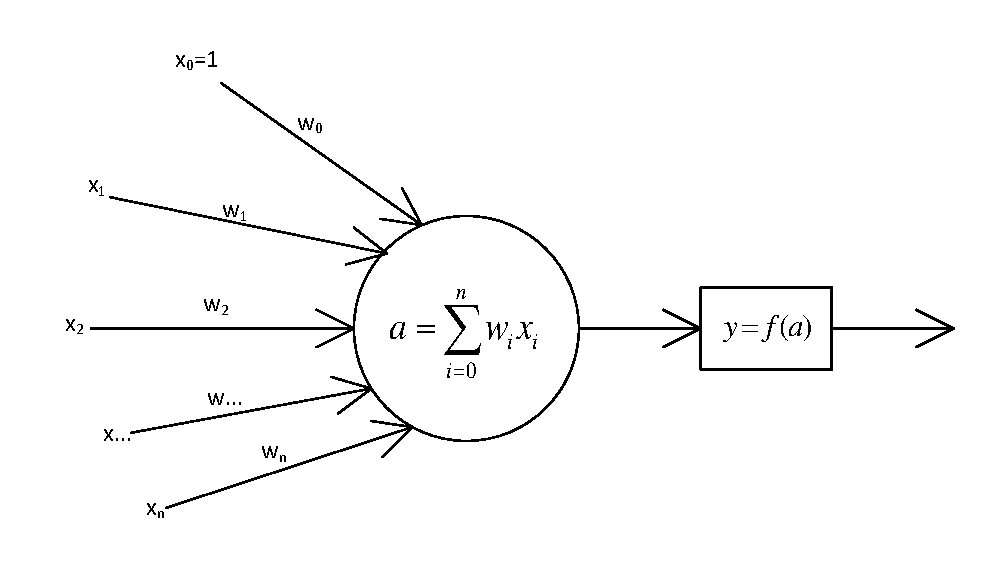
\includegraphics[scale=0.75]{diagrams/1_neuron}
	\caption{Dirbtinis neuronas}
	\label{fig:neuron}
\end{figure}

Dirbtinis neuronas generuoja išeinamąjį signalą pagal tam tikrą modelį.
Skaičiuojant neurono generuojamą signalą, kiekvienos įeinančiosios jungties $k$, turinčios svorį $w_k$ ir ja sklindantį signalą $x_k$ dydžio, šie du dydžiai yra sudauginami.
Tada visos šios signalų dydžių ir svorių sandaugos yra susumuojamos - taip gaunamas sužadinimo signalas $a$ (\ref{eq:a}~formulė).
Tada sužadinimo signalas $a$ yra paduodamas kaip argumentas tam tikrai funkcijai $f$ ir gaunamas neurono išeities signalas $y = f(a)$.
Šį funkcija $f$ yra vadinama aktyvacijos funkcija - ją galima pasirinkti pagal tai, kokio tikslo siekiama iš šio dirbtinio neurono.
Populiariausios aktyvacijos funkcijos - slenkstinė, tiesinė, hiperbolinis tangentas bei sigmoidinė, esanti \ref{eq:sigmoid}~formulėje.
Iš esmės akvyvacijos funkcija gali būti bet kokia funkcija, tačiau vėliau norint apmokyti dirbtinį neuronų tinklą, reikia rasti šios funkcijos išvestinę.
Dėl šios priežasties dažniausiai pasirenkamos tokios aktyvacijos funkcijos, kurios ne tik tinkamai pertvarko signalą išvedimui, tačiau ir kurios išvestinės yra paprastos.

\begin{equation} \label{eq:a}
a = \sum_{k=1}^N w_kx_k
\end{equation}

\begin{equation} \label{eq:sigmoid}
f(a) = \frac{1}{1 + e^{-a}}
\end{equation}

Įeinamosios neurono jungtys numeruojamos nuo 1 iki $k$.
Norint $a$ reikšmę padaryti tinkamesnę neuroninio tinklo funkcijoms, dažniausiai įvedama papildoma $0$-inė jungtis su svoriu $w_0$ ir signalo stiprumu $x_0 = 1$.
Tokiu būdu prie $a$ (formulė~\ref{eq:a}) reikšmės papildomai pridedama $w_0 * x_0 = w_0$ reikšmė.
Šis papildomas narys leidžia koreguoti neurono generuojamą signalą nepriklausomai nuo įeinančių jungčių signalų.



\subsection{Dirbtinių neuronų tinklas}

Dirbtinių neuronų tinklas (angl.~\textit{Artificial neural network}) - tai tinklas, kurį sudaro dirbtiniai neuronai bei jungtys, jungiančios kai kuriuos dirbtinius neuronus.
Per kiekvieną jungtį gali eiti signalas, kuris perduoda vieno neurono išeinamąjį signalą kitam neuronui.
Kiekvienas neuronas gali turėti bet kokį skaičių įeinančių ir bet kokį skaičių išeinančių jungčių.

Kai kurios jungtys gali būti prijungtos tik prie vieno neurono.
Jungtys, kurios įeina į neuroną tačiau neišeina iš jokio neurono, gali būti naudojamos duomenų perdavimui - šiomis jungtimis neuronų tinklui perduodami signalai, atitinkantys duomenis.
Jungtys, išeinančios iš neurono tačiau neįeinančios į jokį neuroną, naudojamos rezultato gavimui - kai per visą neuroninį tinklą pereina signalai, būtent šiose jungtyse ir yra gaunamas pateiktus duomenis atitinkantis atsakymas.

Dirbtinio neuronų tinklo užduotis - pagal pateikiamus duomenis sugeneruoti atsakymą.
Pirmiausia duomenys pateikiami per tam skirtas jungtis.
Neuronai, prijungti prie šių jungčių, gauna šiuos pradinius signalus, juos apdoroja ir pradeda skleisti tam tikro stiprumo signalą išeinančiomis jungtimis.
Taip signalai sklinda tolyn ir visi tinklo neuronai būna apdorojami tol, kol galiausiai rezultatas būna gaunamas tam skirtose jungtyse.



\subsection{Daugiasluoksnis perceptronas}

Daugiasluoksnis perceptronas (angl.~\textit{Multilayer perceptron}) - tai tam tikromis savybėmis pasižymintis dirbtinių neuronų tinklas.
Tai viena populiariausių dirbtinių neuroninių tinklų rūšis, kadangi savybės, kuriomis šis tinklas pasižymi, leidžia padaryti tam tikras skaičiavimo optimizacijas bei pakankamai lengvai realizuoti veikiantį neuroninį tinklą.
Be to, galima keisti daugiasluoksnio perceptrono parametrus pritaikant jį konkrečiai sprendžiamai problemai.

Neuronų tinklą galima nagrinėti kaip grafą, kuriame dirbtiniai neuronai yra grafo viršūnės, o jungtys, jungiančios juos - kryptinės grafo briaunos.
Jeigu neuronų tinklo grafe būtų bent vienas ciklas, tai reikštų, kad šiame cikle esančiomis jungtimis einantys signalai gali keistis ne kartą - atnaujinus tam tikro neurono išvedimo signalą, ciklu gali pakisti ir šio neurono įvedimo signalas.
Tada reikėtų vėl atnaujinti šio neurono išvedimo signalą, o tai darant vėl gali pasikeisti bet kuris ivedimo signalas ir toks pasikeitimų ciklas gali kartotis labai daug kartų arba net ir niekada nesibaigti.
Tai apsunkina dirbtinių neuronų veikimą, todėl dažniausiai naudojami neuronų tinklai, kuriais signalai skleidžiami pirmyn (angl.~\textit{Feedforward}).
Pagal apibrėžimą, jeigu tinklo grafe nėra nei vieno ciklo, tinklas yra pirmyn skleidžiamas.

Tai, kad daugiasluoksnis perceptronas yra skleidžiamas pirmyn, suteikia nemažai privalumų.
Norint apdoroti tam tikrą neuroną, privalu žinoti visus įeinančiųjų jungčių signalų dydžius, o tai reiškia, kad jau turi būti apdoroti visi neuronai, kurių išeinamosios jungtys įeina į apdorojamąjį neuroną.
Grafe be ciklų rasti tokią neuronų seką, kuria būtų galima apdoroti tinklo neuronus nėra sunku - šį užduotis yra plačiai žinoma ir vadinama topologiniu rikiavimu.
Yra žinoma, kad beciklį grafą visada galima topologiškai išrikiuoti, o tai reiškia, kad daugiasluoksnį perceptroną galima apdoroti tiesiog paeiliui apdorojant topologiškai išrikiuotų viršūnių seką.
Šį savybė palengvina neuroninio tinklo apdorojimą.

\begin{figure}
	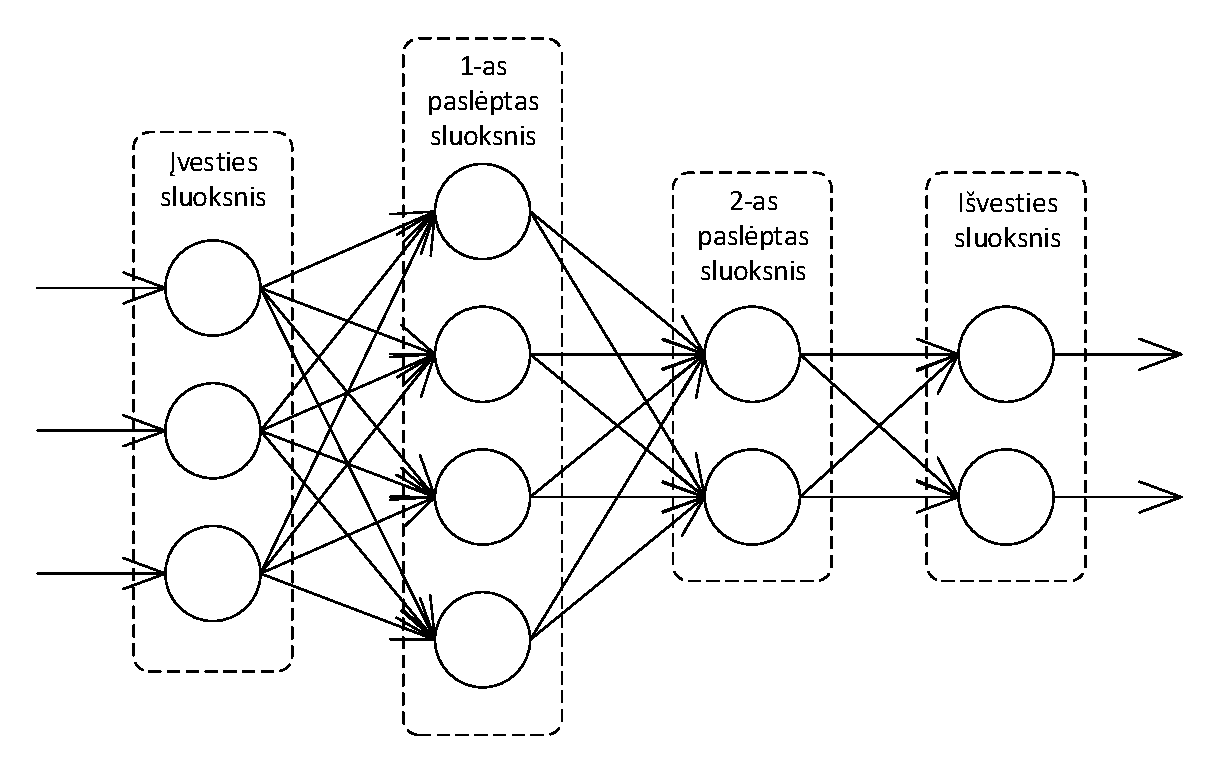
\includegraphics[scale=0.75]{diagrams/2_neural_network}
	\caption{Daugiasluoksnis perceptronas}
	\label{fig:neural_network}
\end{figure}

Be to, daugiasluoksniai perceptronai yra organizuojami sluoksniais (žr. \ref{fig:neural_network} paveiksliuką).
Tinklas yra sudarytas iš perceptronų grupių, kurios yra vadinamos sluoksniais.
Visi neuronų sluoksniai yra išsidėstę iš eilės, nuo kairės į dešinę.
Kiekvieno sluoksnio visi neuronai turi išeinamąsias jungtis į visus neuronus iš sekančio sluoksnio, esančio dešinėje.
Išimtis paskutinis sluoksnis, vadinamas išvesties sluoksniu (angl.~\textit{Output layer}) - kadangi jis naudojamas išvedimui, todėl neturi jungčių į kitus neuronus, o jo jungtyse formuojamas atsakymas į analizuojamą problemą.

Pirmasis neuronų sluoksnis, kuriam paduodami duomenys, vadinamas įvesties sluoksniu (angl.~\textit{Input layer}).
Po to gali būti vienas ar keli paslėpti sluoksniai (angl.~\textit{Hidden layer}), kurie naudojami tam, kad neuroninio tinklo struktūra būtų didesnė ir to pasekoje gebėti išmokti sudėtingesnius dalykus.
Paprasčiausiuose tinkluose gali išvis nebūti paslėptų sluoksnių, tačiau tokio tinklo galimybės būtų labai ribotos ir jo apmokymas sudėtingesnėms užduotims užtruktų daug ilgiau.
\TODO{įdėti ref į straipsnį apie SLP lėtą mokymasi sunkioms užduotims - iš dėstytojo}
Paskutinysis sluoksnis, naudojamas rezultatų suformavimui, vadinamas išvesties sluoksniu.

Tokia neuronų organizacija į sluoksnius dar palengvina tinklo veikimą - signalus siųsti galima sluoksnis po sluoksnio, pradedant pirmuoju, kuris gauna problemos duomenis, siunčiant signalus visomis jungtimis antrąjam sluoksniui.
Po to tas pats atliekama su antruoju sluoksniu siunčiant visus signalus trečiąjam ir t.t., kol galiausiai rezultatai gaunami paskutiniame sluoksnyje.

Savybė, kad kiekvieno sluoksnio, išskyrus paskutinio, visi neuronai turi išeinamąsias jungtis į visus sekančio sluoksnio neuronus taip pat yra naudinga - žinant tai, nereikia turėti jokio tinklo grafo, kadangi užtenka žinoti kiekvieno sluoksnio neuronus bei jungčių svorius.
Be to, signalų siuntimas iš vieno sluoksnio į sekantį taip pat gali būti suprastintas.
Vietoj to, kad programiškai iteruoti per visas dviejų sluoksnių neuronų poras ir atlikti jungties dydžio skaičiavimą, tą galima padaryti su matricų aritmetika.
Signalo skaičiavimo atliekamas operacijas, nurodytas \ref{eq:a} formulėje, galima sutraukti į matricų daugybos operacijas, o aktyvacijos funkciją pritaikyti visai matricai.
Taip daugiasluoksnio perceptrono tinklo modelis tampa dar tvarkingesnis ir paprastesnis.


\TODO{citata?}

\TODO{110 iš knygos}

\TODO{Perkelti statinės struktūros aprašymą (pateiktą žemiau):}

Projektuojant daugiasluoksnį perceptroną konkrečiam uždaviniui, reikia parinkti jo struktūrą.
Reikia nuspręsti, kiek neuronų sluoksnių bus, kiek kiekviename sluoksnyje bus neuronų, kokios aktyvacijos funkcijos bus naudojamos, kaip duomenys yra paduodami, kokiu formatu iš tinklo gaunami rezultatai.
Norint efektyviai spręsti konkretų uždavinį, labai svarbu parinkti tinkamą struktūrą.
Nuo parinktos struktūros priklauso daugiasluoksnis perceptronas galimybės mokytis - parinkus blogą struktūrą, tinklas gali nesugebėti išmokti sudėtingesnių duomenų atvejų.



\subsection{Neuroninio tinklo apmokymas} \label{network-learning}

%Neuronų tinklo pateiktas atsakymas nebūtinai yra teisingas - neuronų tinklas suprojektuotas taip, kad jį būtų galima tobulinti pagal daromas klaidas.

Daugiasluoksnis perceptronas suprojektuotas taip, kad pagal mokymui naudojamus duomenis jis galėtų būti keičiamas ir jo pateikiami atsakymai panašėtų į teisingus.
%Pagal tinklo pateiktą rezultatą ir iš anksto žinomo rezultato skirtumus keičiami jungčių svoriai taip, kad kitą kartą būtų gaunamas atsakymas, artimesnis teisingui.
%Neuroniui tinklui pateiktus neteisingą atsakymą, vykdomas tinklo mokymas.
Vienas populiariausių mokymo metodikų, kuri yra naudojamas šiame darbe - atgalinė propogacija (angl.~\textit{Backpropogation}).
Tam, kad būtų galima apmokyti neuronų tinklą spręsti konkrečią problemą, reikia turėti nemažą šios problemos pavyzdinių duomenų rinkinį bei iš anksto žinoti kiekvienų duomenų teisingą atsakymą.
Mokymas vyksta pažingsniui, vienu metu neuroninui tinklui pateikiant vienus duomenis iš turimo duomenų rinkinio.
Neuroninis tinklas, gavęs duomenis, juos analizuoja ir pateikia tam tikrą atsakymą.
Šis gautas atsakymas yra sulyginamas su teisingu, iš anksto žinomu atsakymu.
Pagal tai, kaip neurininio tinklo pateiktas atsakymas skiriasi nuo teisingojo, neuroninis tinklas būna pertvarkomas.
Pertvarkymas vyksta nagrinėjant neuroninį tinklą pradedant nuo paskutinio sluoksnio ir baigiant pirmuoju - t.y. priešinga tvarka, nei buvo nagrinėjama, kai neuroninis tinklas analizavo pateiktus duomenis.
Nagrinėjant kiekvieną neuroninio tinklo neuroną, į jį įeinančių jungčių svoriai $w_k$ (įskaitant ir $w_0$, kuris naudojamas kaip papildomas parametras) būna pakeičiami taip, kad neuroninis tinklas gautų panašesnį atsakymą į teisingąjį.

Lyginant tinklo pateiktą atsakymą su teisingu, būna apskaičiuojama atsakymo klaida, pateikta \ref{eq:error}~formulėje.
Čia $r$ - teisingo, iš anksto žinomo atsakymo vektorius, $a$ - neurono pateikto atsakymo vektorius, o N - vektorių dydis.

\begin{equation} \label{eq:error}
E = \frac{1}{N} \sum_{k=1}^N (r_k - a_k)^2
\end{equation}

Ši klaida parodo, kiek atsakymas yra klaidingas.
Didesnė klaida reikškia neteisingesnį atsakymą, todėl apmokant tinklą tikslas yra minimizuoti šią klaidą.
Tai pasiekiama analizuojant, kaip kiekvienas jungčių svoris prisideda prie klaidos - apskaičiuojamos klaidos išvestinės pagal kiekvieną svorį ir svoriai yra keičiami taip, kad klaida mažėtų (\ref{eq:learning}~formulė).
Šioje formulėje yra panaudojamas $\eta$ mokymo koeficientas - jis nulemia, kaip greitai tinklas mokosi.
Parinkus per mažą mokymo koeficientą, mokymo procesas bus lėtas ir geram apmokymui reikės daug iteracijų, o perinkus per didelį - mokymo metu tinklo svoriai bus per daug keičiami ir taip nesugebės efektyviai tobulėti.
Mokymo koeficientas parenkamas priklausomai nuo konkrečios sprendžiamos užduoties bei tinklo struktūros.
Dažniausiai jis parenkamas bandymų metu, išbandant įvairius dydžius.

\begin{equation}\label{eq:learning}
w' = w - \eta\frac{\partial E}{\partial w}
\end{equation}

Taip atlikus vienų rinkinio duomenų apmokymą, imami kiti duomenys iš šio rinkinio ir mokymas kartojamas.
Kiekvienus duomenis iš šio rinkinio rekomenduotina naudoti apmokymui bent kelis kartus, kadangi neuroninis tinklas ne iš karto teisingai išmoksta spręsti problemą su konkrečiais duomenimis.
Taip pat apmokant tinklą su vienais duomenimis, neuroninio tinklo svoriai gali būti pakeisti taip, kad neuroninis tinklas nebegebės teisingai išspręsti prieš teisingai išspręstų duomenų.


%Neuroninių tinklų mokymo principas yra apmokyti jį mokant vieno pavyzdžio vienu metu.
%Pavyzdžio duomenys būna paduodami tinklui, gaunamas konkretus atsakymas, kuris yra sulyginamas su teisingu atsakymu.
%Pagal tai, koks buvo gautas atsakymas ir koks yra teisingas atsakymas, apskaičiuojama, kaip reikia pakeisti tinklo svorius, kad kitą kartą būtų gautas atsakymas, panašesnis į teisingą.
%Tai pasiekiama kiekvienam tinklo svoriui apskaičiavus, kaip ir kiek jį reikia pakeisti (padidinti ar pamažinti svorį).
%Tuomet koeficientas yra pakeičiamas pagal tai, kaip tuo metu jo pakeitimas pakeistų analizuojamo pavyzdžio atsakymą.



\subsection{Neuroninio tinklo persitaikymas}

%Tačiau per daug mokyti neuroninį tinklą taip pat nerekomenduotina, kadangi vėliau tinklas per daug prisitaiko prie jam apmokyti naudojamo duomenų rinkinio, o ne prie problemos.
%Nors ir gali pasirodyti, kad neuroninio tinklo pateikiami rezultatai vis labiau ir labiau panašėja į teisingus, tačiau išbandžius šį neuroninį tinklą su kitu šios problemos duomenų rinkiniu galima įsitikinti, kad rezultatai po kurio laiko pradeda blogėti.

Apmokant neuroninį tinklą gan svarbu nuspręsti, kada apmokymą reikia nutraukti, kadangi per daug mokyti neuroninį tinklą taip pat nėra naudinga.
Atliktame tyrime \cite[114~psl.]{overfitting} aptariama, kodėl per daug mokant daugiasluoksnį perceptroną siekiant minimizuoti mokymo klaidą rezultatai su kitais, mokymui nepanaudotais duomenimis, gali pablogėti.
Neuroniniai tinklai mokymo procese yra linkę prisitaikyti prie konkrečių mokymui naudojamų duomenų.
Taip atsitinka todėl, kad neuroninio tinklo gerumas yra matuojamas pagal tai, kokios klaidos gaunamos naudojant mokymui parinktus duomenis.
Kadangi mokymui yra naudojama baigtinė aibė duomenų, todėl neuroninis tinklas stengiasi kuo labiau prie jų visų prisitaikyti, neatsižvelgdamas į tai, kad gali egzistuoti ir kitokie duomenys.
Dėl to po tam tikro skaičiaus mokymo įtaracijų dažnai įvyksta persitaikymas (angl.~\textit{Overfitting}) - neuroninis tinklas siekia sumažinti mokomų duomenų pateikiamą klaidą taip stipriai, kad nuo to gali kentėti kitų, ne iš mokymo aibės pateikiamų įrašų atsakymai.

Viena priežastis, kodėl taip įvyksta - ne visi duomenys tobulai atitinka analizuojamą populaiciją. Dažniausiai duomenyse egzistuoja tam tikros anomalijos, būdingos tik keliems duomenų įrašams, kurios pirmiausia būna natūraliai ignoruojamos.
Nors ir gaunamas blogas atsakymas su tokiomis anomalijomis, visgi tokių įrašų yra mažuma, todėl bendras rezultatas yra neblogas.
Atliekant daugybę itaracijų su tais pačiais mokymo duomenimis, neuroninis tinklas pasiekia tokį atsakymų tikslumą, kad norint dar bent kiek patobulėti, reikia prisitaikyti prie šių anomalijų, kadangi ir jos didina neuroninio tinklo klaidą.
Tada neuroninio tinklo struktūra keičiasi taip, kad apimtų ir šią anomaliją, tačiau dėl to kenčia likusios problemos populiacijos, neįeinančios į apmokymo rinkinį, rezultatai.

Kita priežąstis, dėl kurios įvyksta persitakymas, yra lokalių minimumų problema.
Prieš pradedant neuroninio tinklo apmokymą, visi neuronų jungčių svoriai yra parenkami atsitiktinai.
Dėl to gaunamas atsitiktinis neuroninis tinklas, kuris jau pateikia tam tikrus atsakymus.
Tikėtina, kad jo pateikiami atsakymai yra labai prasti ir gali būti pagerinti, kadangi tai visiškai naujas atsitiktinai sukurtas tinklas, dar nieko nežinantis apie tiriamą problemą.
Dėl to mokymo metu jis tobulėja, mažindamas mokymo duomenų pateikiamą klaidą.
Problema kyla dėl to, kad neuroninio tinklo tobulėjimas vyksta mažais žingsniais, iš dabartinių turimų svorių juos keičiant po truputį taip, kad atsakymas pagerėtų.
O kadangi visas mokymas prasideda nuo atsitiktinai sugeneruotų duomenų, todėl pats mokymas bus ne artėjimas prie idealaus tinklo, o prie panašaus į atsitiktinį tinklą, kuris veiktų geriau, nei dabar.
Tačiau kartais norint pasiekti gerų rezultatų, gali prireikti drąstiškai pakeisti daugybę tinklo svorių vienu metu.
Visgi to tinklas padaryti negali, nes vienu metu jis analizuoja tik vieną duomenų įrašą, neatsižvelgiant apie kitus, todėl rimtesni pakeitimai sugadintų neuroninį tinklą sprendžiant tiriamą problemą.
Dėl to apmokomas tinklas turi ribas, iki kiek iš tikro gali tobulėti - ši riba ir yra vadinama lokaliu minimumu.
Artėdamas prie lokalaus minimumo, tinklas taip stipriai prisiderina prie mokymui panaudotų duomenų, kad jo struktūros teikiami rezultatai taip pat pradeda blogėti tiriamajai problemos populiacijai.

Paskutinė persitaikymo priežąstis, kuri šiek tiek paaiškina prieš tai buvusias priežąstis, yra ta, kad neuroninis tinklas vėlesnėse iteracijose per daug siekia tobulumo.
Dažnai maža neuroninio tinklo pateikiama klaida nereiškia blogo atsakymo.
Klasifikavimo uždavinyje atsakymas yra grupė, kuriai analizuojamas įrašas priklauso.
\TODO{pridėti ref į klasifikavimo tinklo aprašymą?}
Tačiau jo pateikiamo atsakymo formatas skiriasi - atsakyme yra gaunama, kiek šis įrašas turi kiekvienos grupės savybių.
Iš šio tinklo pateikiamo atsakymo rezultatas gaunamas išrenkant grupę, kuri yra būdingiausia įrašui.
Dėl to atsakymas būtų idealus, jeigu analizuojamas įrašas būtų 100\% priklausomas grupei, kuriai jis priklauso, ir 0\% kitoms.
Tačiau dažnai netgi patys duomenys gali būti tokios prigimties, kad nors jie ir priklauso vienai konkrečiai grupei, visgi turi ir kitų grupių savybių.
Dėl to siekis, kad kiekvienas mokymo duomenų įrašas būtų pripažintas kaip 0\% priklausomas kitoms grupėms, šiek tiek kenkia tinklo tobulėjimui - nors ir pasiekiamas teisingas atsakymas, visgi bandoma jį vis tobulint, siekiant pasiekti 0\% ir 100\% priklausomybę atitinkamoms grupėms.
Čia ir įvyksta persitaikymas, nes po tam tikro iteracijų skaičiaus neuroninis tinklas tiek bando pasiekti minimalią galima klaidą, kad jo rezultatas su likusia problemos duomenų populiacija pradeda kristi.

Norint gauti neuroninį tinklą, kuris teisingai spręstų ne tik mokymui parinktus duomenis, bet ir likusią problemos duomenų populiaciją, reikia vengti persitaikymo.
Tą galima padaryti naudojant validacijos rinkinį (angl.~\textit{Validation set}).
Apmokymui reikia parinkti ne tik apmokymui naudojamą rinkinį, bet taip pat ir validacijos rinkinį.
Šie duomenų rinkiniai turi neturėti bendrų įrašų, priešingu atveju validacija nebus veiksminga.
Taip pat tiek apmokymo, tiek validacijos rinkiniuose turėtų būti kuo įvairesnių ir skirtingesnių įrašų - jie turi apimti įvairius skirtingus duomenų variantus tam, kad neuroninis tinklas juos išmoktų bei kad validacija būtų efektyvi.
Turint apmokymo ir validacijos rinkinius, apmokymas vyksta įprastai - tinklas mokomas spręsti po vieną įrašą.
Tačiau vietoj to, kad tinklo progresas būtų sekamas pagal tai, kaip gerai ji sprendžia apmokymo rinkinį, yra panaudojamas validacijos rinkinys.
Po kiekvienos apmokymo iteracijos, neuroniniui tinklui yra duodami validacijos rinkinio įrašai.
Juos neuroninis tinklas turi išspręsti, tačiau be mokymosi žingsnio, nes kitaip validacijos rinkinys netektų prasmės.
Gavus validacijos rinkinio atsakymų klaidą, ją galima naudoti stebint neuroninio tinklo progresą.
Paprastai mokymo pradžioje validacijos rinkinio klaida mažėja kartu su mokymo rinkinio klaida, tačiau po tam tikro iteracijų skaičiaus ši klaida gali pradėti didėti, nors apmokymo rinkinio gaunama klaida vis dar mažėja.
Būtent šioje vietoje ir prasideda persitaikymas, todėl vos pasiekus šią ribą arba dar po kelių iteracijų nuo jos geriausia neurono apmokymą nutraukti.

\TODO{paieškoti lokalių minimumų straipsnių}



\subsection{Momento koeficientas}

Momento koeficientas - tai itin populiari neuroninio tinklo modifikacija, skirta pagerinti tinklo mokymosi procesą.
Ji remiasi \ref{network-learning} poskiryje aprašytu mokymu, tačiau šiek tiek praplečia svorių keitimą.
Svoriai keičiami ne pagal \ref{eq:learning} formulę, o pagal jos plėtinį \ref{eq:moment-2} formulėje.

Svoriai keičiami ne tik pagal tai, kaip svorius keisti apsimoka būtent šiuo metu būtent šiam testui, tačiau ir pagal tai, kaip tai buvo keičiama praeitose mokymo iteracijose.
Tai įgyvendinama pasinaudojant greičio ir įveikto atstumo fizikinį analogą - kai norima įveikti tam tikrą atstumą, kūnui reikia suteikti jėgos ir įgauti greitį, o greitis leis judėti.
Panašiai veikia momento koeficientas - analizuojant, kaip reikia pakeisti svorius, šie dydžiai nėra tiesiog pritaikomi šiuo metu, tačiau jie yra panaudojami kaip greitis - svorio kitimo žingsnis.
Kiekvienam svoriui išsaugomas kitimo žingsnis, aprašytas \ref{eq:moment-1} formulėje, kuris po kiekvienos apmokymo iteracijos pakeičiamas padidinant ar pamažinant tam tikra reikšme pagal tai, kaip šioje iteracijoje reikia keisti svorio dydį.
Šis turimas žingsnis kiekvienos iteracijos metu yra pritaikomas kaip pokytis svoriui keisti.

\begin{equation} \label{eq:moment-1}
v' = \mu v - \eta \frac{\partial C}{\partial w}
\end{equation}

\begin{equation} \label{eq:moment-2}
w' = w + v'
\end{equation}

Toks svorių keitimo metodas suteikia kelis privalumus.
Pirmiausia, mokymo procesas pagreitėja - jei kelias iteracijas svorį reikia keisti ta pačia linkme, naudojant šį metodą prireiks mažiau iteracijų, kadangi pakeitimas sumuosis ir kaskart bus panaudojamas vis didesnis pakeitimo žingsnis.
To pasiekti vien padidinus mokymo koeficientą nepavyks, kadangi didelis mokymo koeficientas atliks didelius pakeitimus net ir ten, kur jų nereikia.
Tuo tarpu naudojant momento koeficientą, mokymas prasidės mažais žingsniais ir jeigu mokymo kryptis pasikeis, taip pat pradės keistis ir svorio keitimo žingsnis.

Taip pat šis metodas leidžia išvengti dalies lokalių minimumų.
Tai įvyksta natūraliai, kadangi įgavus pakankamai didelį svorio keitimo žingsnį, patekimas mažą į lokalų minimumą nesugebės greitai pakeisti svorio keitimo krypties.
Žinoma, lokalus minimumas turės įtakos svorio keitimo žingsniui, tačiau jeigu šis lokalus minimumas yra pakankamai mažas ir nereikšmingas, tada turimas svorio keitimo žingsnis leis kurį laiką tęsti svorio keitimą į tą pusę, į kurią jis buvo keičiamas senesnėse iteracijose.

\TODO{see commented line - url for reference}
%http://ieeexplore.ieee.org/xpl/login.jsp?tp=&arnumber=4579193&url=http%3A%2F%2Fieeexplore.ieee.org%2Fiel5%2F4569827%2F4579133%2F04579193.pdf%3Farnumber%3D4579193

%Tinklo apmokymui naudojamas apmokymo rinkinys, sudarytas iš kelių (dažniausiai daugybės) skirtingų įrašų.
%Naudojant paprastą apmokymo metodą, kiekvieno įrašo apmokymas yra atskiras procesas.
%Naudojant momento koeficientą, svorių keitimo tendencijos tarp skirtingų įrašų išlieka.
%Tai suteikia tam tikro pranašumo, kadangi labai išsiskiriantys ar nevisai korektiški įrašai, kurių paprastai yra nedaug, mažiau neigiamai paveiks tinklą.
%Taip yra todėl, kad jie keis ne pačias svorio reikšmes, bet greitį, kuris yra priklausomas ir nuo senesnių kitų įrašų iteracijų.
%Tai gali padėti išvengti tinklo pakeitimo tokia linkme, kuri kitiems įrašams gali stipriai pabloginti rezultatą - pavyzdžiui, patekimo į lokalų minimumą.



\section{Duomenys}

\TODO{duomenų įžanga}


\subsection{Vilkdagių duomenys}

Programuojant daugiasluoksnį perceptroną, testavimui buvo panaudoti vilkdagių (angl.~\textit{Iris flower}) duomenys.
Tai plačiai taikomi ir viešai prieinami duomenys, aprašantys 3 rūšių vilkdagius.
Aprašyta po 50 kiekvienos rūšies vilkdagių.
Kiekvienas vilkdagis aprašomas pateikiant 4 dydžius: taurėlapio ilgį, taurėlapio plotį, vainiklapio ilgį bei vainiklapio plotį.
Taigi šiuos vilkdagių duomenis sudaro 150 gėlių, kurių kiekviena aprašyta 4 parametrais bei priskirta vienai iš 3 vilkdagių grupių.

Šie duomenys puikiai tinka klasifikavimo tinklo apmokymui - tinklo tikslas yra kuo mažiau klystant pasakyti, kuriai iš 3 rūšių vilkdagis su tam tikrais parametrais priklauso.
Be to, yra pakankamai duomenų, kad būtų galima dalį jų panaudoti tinklo apmokymui, o kitą dalį - validavimui ir testavimui.
Tokiu būdu galima patikrinti, ar tinklas teisingai išmoko atskirti vilkdagių rūšis pagal parametrus, o ne tiesiog prisitaikė prie mokymui panaudotų duomenų.



\subsection{Biomedicininiai duomenys}

Tyrimui buvo naudojami biomedicininiai chromosomų duomenys, naudoti \cite[289~psl.]{price-dimensionality-reduction} tyrime.
Kiekvieną chromosomą aprašo 30 parametrų.
Visos chromosomos priklauso vienai iš 24 grupių, ir kiekvienoje grupėje yra po 500 chromosomų, taigi visus duomenis sudaro 12000 chromosomų.
Chromosomų parametrų reikšmės yra natūralieji skaičiai.
Šie duomenys tinkami tiriamajai problemai, kadangi jie yra klasifikuojami, turi nemažai parametrų bei kiekvienoje grupėje yra pakankamai duomenų.



\subsection{Duomenų normavimas}

Analizuojami duomenų parametrai gali būti labai skirtingi, kadangi jie išreiškia skirtingas savybes, dydžius, yra išreikšti skirtingais vienetais.
Skiriasi parametrų mąsteliai - pvz. vieno parametro reikšmės gali kisti intervale $[0; 10]$, o kito $[10^3; 10^9]$.
Dėl šių skirtumų tokias parametrų reikšmes tiesiai pateikti neuroniniui tinklui nėra praktiška.
Taip atsitinka dėl neuroninio tinklo veikimo principo - parametrai, kurių reikšmės linkusios būti didesnėmis, turėtų didesnę įtaką rezultatui nei parametrai su mažesnėmis reikšmėmis, kadangi pradiniai duomenų signalai būtų daug stipresni parametrų su didesnėmis reikšmėmis.
Tačiau daug naudingiau būtų visiems parametrams suteikti vienodą svarbą, kadangi parametro reikšmių intervalas neturi nieko bendro su parametro svarba - gali būti ir taip, kad dideles reikšmes įgyjantis parametras yra kur kas mažiau svarbus nei mažas reikšmes įgyjantysis.
Dėl šios priežasties prieš pateikiant duomenis neuroniniui tinklui, juos svarbu normuoti.

\TODO{add ref about normalization - kodėl ji būtina (dėl skirtingų mąstelių)}

Normuojant duomenis, kiekvienas duomenų parametras normuojamas atskirai.
Norint sunormuotį parametrą, reikia išnagrinėti turimas šio parametro reikšmes bei pakeisti jas naujomis.
Sunormavus duomenis, visi parametrai turėtų turėti beveik lygią svarbą neuroniniui tinklui - jų reikšmių pasiskirstymai bei intervalai turėtų būti apyligiai (priklausomai nuo normavimo metodo).
Paprasčiausias parametro normavimo metodas - rasti minimalią $p_{min}$ ir maksimalią $p_{max}$ parametro reikšmes ir kiekvieną $i$-tojo įrašo analizuojamo parametro reikšmę $p_i$ pakeisti pagal formulę:

\begin{equation}
p_i = \frac{p_i - p_{min}}{p_{max} - p_{min}}
\end{equation}

Šis metodas užtikrina, kad naujos parametro reikšmės būtų intervale $[0; 1]$.
Tai buvo naudojama tyrimo pradžioje, kadangi tai turbūt paprasčiausias ir lengviausiai suvokiamas metodas.
Visgi vėliau buvo pradėtas naudoti kitas metodas, naudotas ir aprašytas \cite{gaussian} šaltinyje - Gauso normavimas (angl.~\textit{Gaussian Normalization}).
Pagal šį metodą, radus parametro vidurkį $p_{mean}$ ir vidutinį nuokrypį $p_{std}$, kiekviena $i$-tojo įrašo analizuojamo parametro reikšmė keičiama pagal formulę:

\begin{equation}
p_i = \frac{p_i - p_{mean}}{p_{std}}
\end{equation}

Šiuo metodu gaunamų reikšmių vidurkis lygus nuliui, o dispersija lygi vienetui.
Nors ir šiuo metodu gaunami duomenys nėra apibrėžti konkrečiame reikšmių intervale kaip pirmojo metodo, visgi vidutiniškai 68\% duomenų reikšmių bus intervale $[-1; 1]$.
Bandymu metu šis metodas pasirodė tinkamesnis tiriamai problemai.

\TODO{pridėti dar vieną interalų grupė su 99.x\% tikimybe}

\TODO{add ref for 68\% - the same ref as in previous paragraph}



\section{Dimensiškumo mažinimas}

Efektyvus dimensiškumo mažinimas šiame tyrime yra labai svarbus, kadangi norint tiksliai ištirti, ar galima pasiekti geresnius klasifikavimo rezultatus mažinant duomenų dimensiškumą, yra kritiškai svarbu kuo tiksliau paruošti kompresuotus duomenis.

\TODO{feature axtraction}

\TODO{removing redundant information (kaip pasimatė vėlesniuose rezultatuose)}

\TODO{big parsity of date with high-dimensional data - reducing dimensionality can decrease the parsity}

\TODO{ref apie feature extraction for classification}

\TODO{egzistuoja daugybė dimensiškumo mažinimo būdų}

\TODO{aptariami keli metodai}



\subsection{Tiesinė diskriminantinė analizė}

Vienas iš galimų dimensiškumo mažinimo sprendimo būdų - tiesinė diskriminantinė analizė (angl.~\textit{Linear discriminant analysis}).

\TODO{Aprašyti veikimą}

Pagrindinis šio metodo suvaržymas yra tai, kad kiekvienas naujas parametras yra gaunamas sudėjus originalių parametrų reikšmes, padaugintas iš atitinkamų koeficientų.
Tai reiškia, kad naujieji parametrai turi tiesinę priklausomybę nuo senųjų, todėl toks dimensijų mažinimas yra labai elementarus.
Jeigu norima sukurti naują parametrą, kurio išvedimas yra sudėtingesnis, to padaryti naudojant šį metodą nepavyks.
Dėl to gaunamos parametrų reikšmės gali būti mažai naudingos.

\TODO{statistinis dimensijų mažinimas - tiesinis (linear), o neuroniniai tinklai geba atlikti sudėtingesnias transformacijas.}

\TODO{paaiškinti, kaip veikia tiesinis - kiekviena nauja savybė gaunama iš originalių savybių su tam tikrais apskaičiuojamais koeficientais.}


\url{http://en.wikipedia.org/wiki/Linear_discriminant_analysis#Face_recognition}

\TODO{Pavyzdinio rezultato paveiksliukas}

\TODO{matlab, python script}


\TODO{SVD? \url{http://en.wikipedia.org/wiki/Singular_value_decomposition}}


\subsection{Dimensiškumo mažinimas daugiasluoksniu perceptronu} \label{dimensionality-reduction-perceptron}

Dimensiškumo mažinimui tyrimo metu buvo panaudotas daugiasluoksnis perceptronas (\ref{fig:compression_perceptron}~pav.).
Turint $N$ dimensijų ir norint jas sumažinti iki $M$, kai $M < N$, tai buvo atliekama sukūrus neuroninį tiklą, kurio pirmajame ir paskutiniajame sluoksniuose yra po $N$ neuronų, o viename iš vidinių sluoksnių - $M$ (šį vidinį sluoksnį vadinkime kompresijos sluoksniu).
Tokio neuroninio tinklo užduotis nėra tiesiog sumažinti dimensijų skaičių - tai daroma netiesiogiai.
Šiam tinklui perduodant tam tikrus $M$ dimensijų turinčius duomenis, iš jo tikimasi, kad išeities neuronuose susiformuos rezultatas, lygus pradiniams duomenims - tai yra neuronų tinklas šių duomenų nepakeis.
Ši užduotis būtų paprasta, jeigu visi vidiniai turėtų bent $N$ dimensijų - tada pateikiami duomenys galėtų būti tiesiog perkeliami iš vieno neuronų sluoksnio į kitą nepakeisti.
Tačiau kompresijos sluoksnis turi tik $M$ neuronų - vadinasi, duomenis reikės tam tikru būdu pertvarkyti, kad jie galėtų būti perduodami per šį sluoksnį prarandant kuo mažiau savybių.
Būtent čia ir įvyksta dimensiškumo mažinimas - neuroninis tinklas yra apmokomas pateikti kuo panašesnius duomenis į pradinius, ko pasekoje kompresijos sluoksnyje su $M$ neuronų yra gaunami duomenys, turintys mažiau dimensijų.
Norint sumažinti tam tikrų duomenenų dimensijas, užtenka šiuos duomenis paduoti apmokytui neuroniniui tinklui ir pažiūrėti, kokie duomenys susidarė kompresijos sluoksnyje.
Nuskaičius šių neuronų reikšmes ir bus gaunami duomenys, turintis mažiau dimensijų.

\begin{figure}
	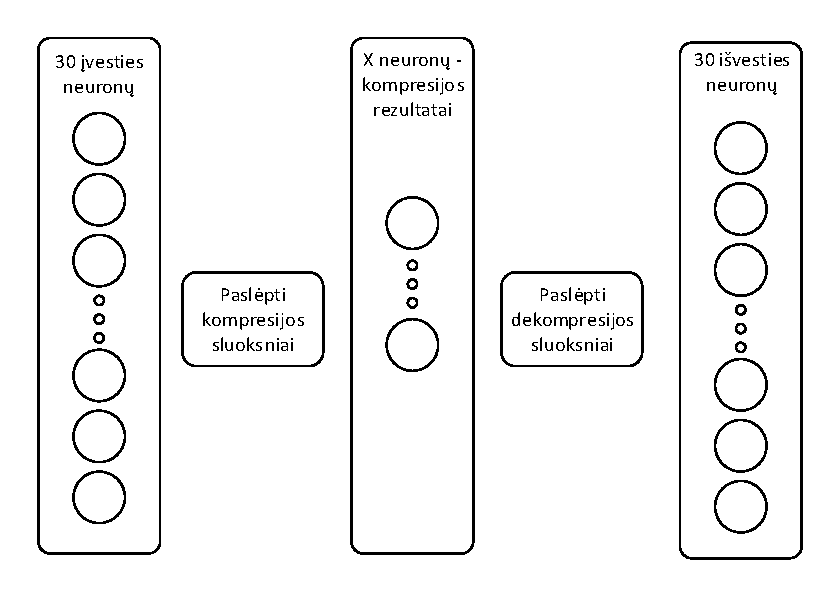
\includegraphics[scale=0.75]{diagrams/compression_perceptron}
	\caption{Dimensiškumo mažinimo perceptrono struktūra}
	\label{fig:compression_perceptron}
\end{figure}

Tokiame apmokytame neuroniniame tinkle visi sluoksniai, esantys kairėje nuo kompresijos sluoksnio, yra naudojami dimensiškumo mažinimui.
Būtent per šiuos sluoksnius einant signalams ir yra sudaromi mažiau dimensijų turintis duomenys.
Kadangi šio neuroninio tinklo tikslas yra pateikti rezultatą, kuris būtų kuo panašesnis į pateiktus duomenis, todėl galima teikti, kad sluoksniai, esantys dešinėje nuo kompresijos sluoksnio, yra naudojami pradinių duomenų dekompresijai.

\begin{figure}
	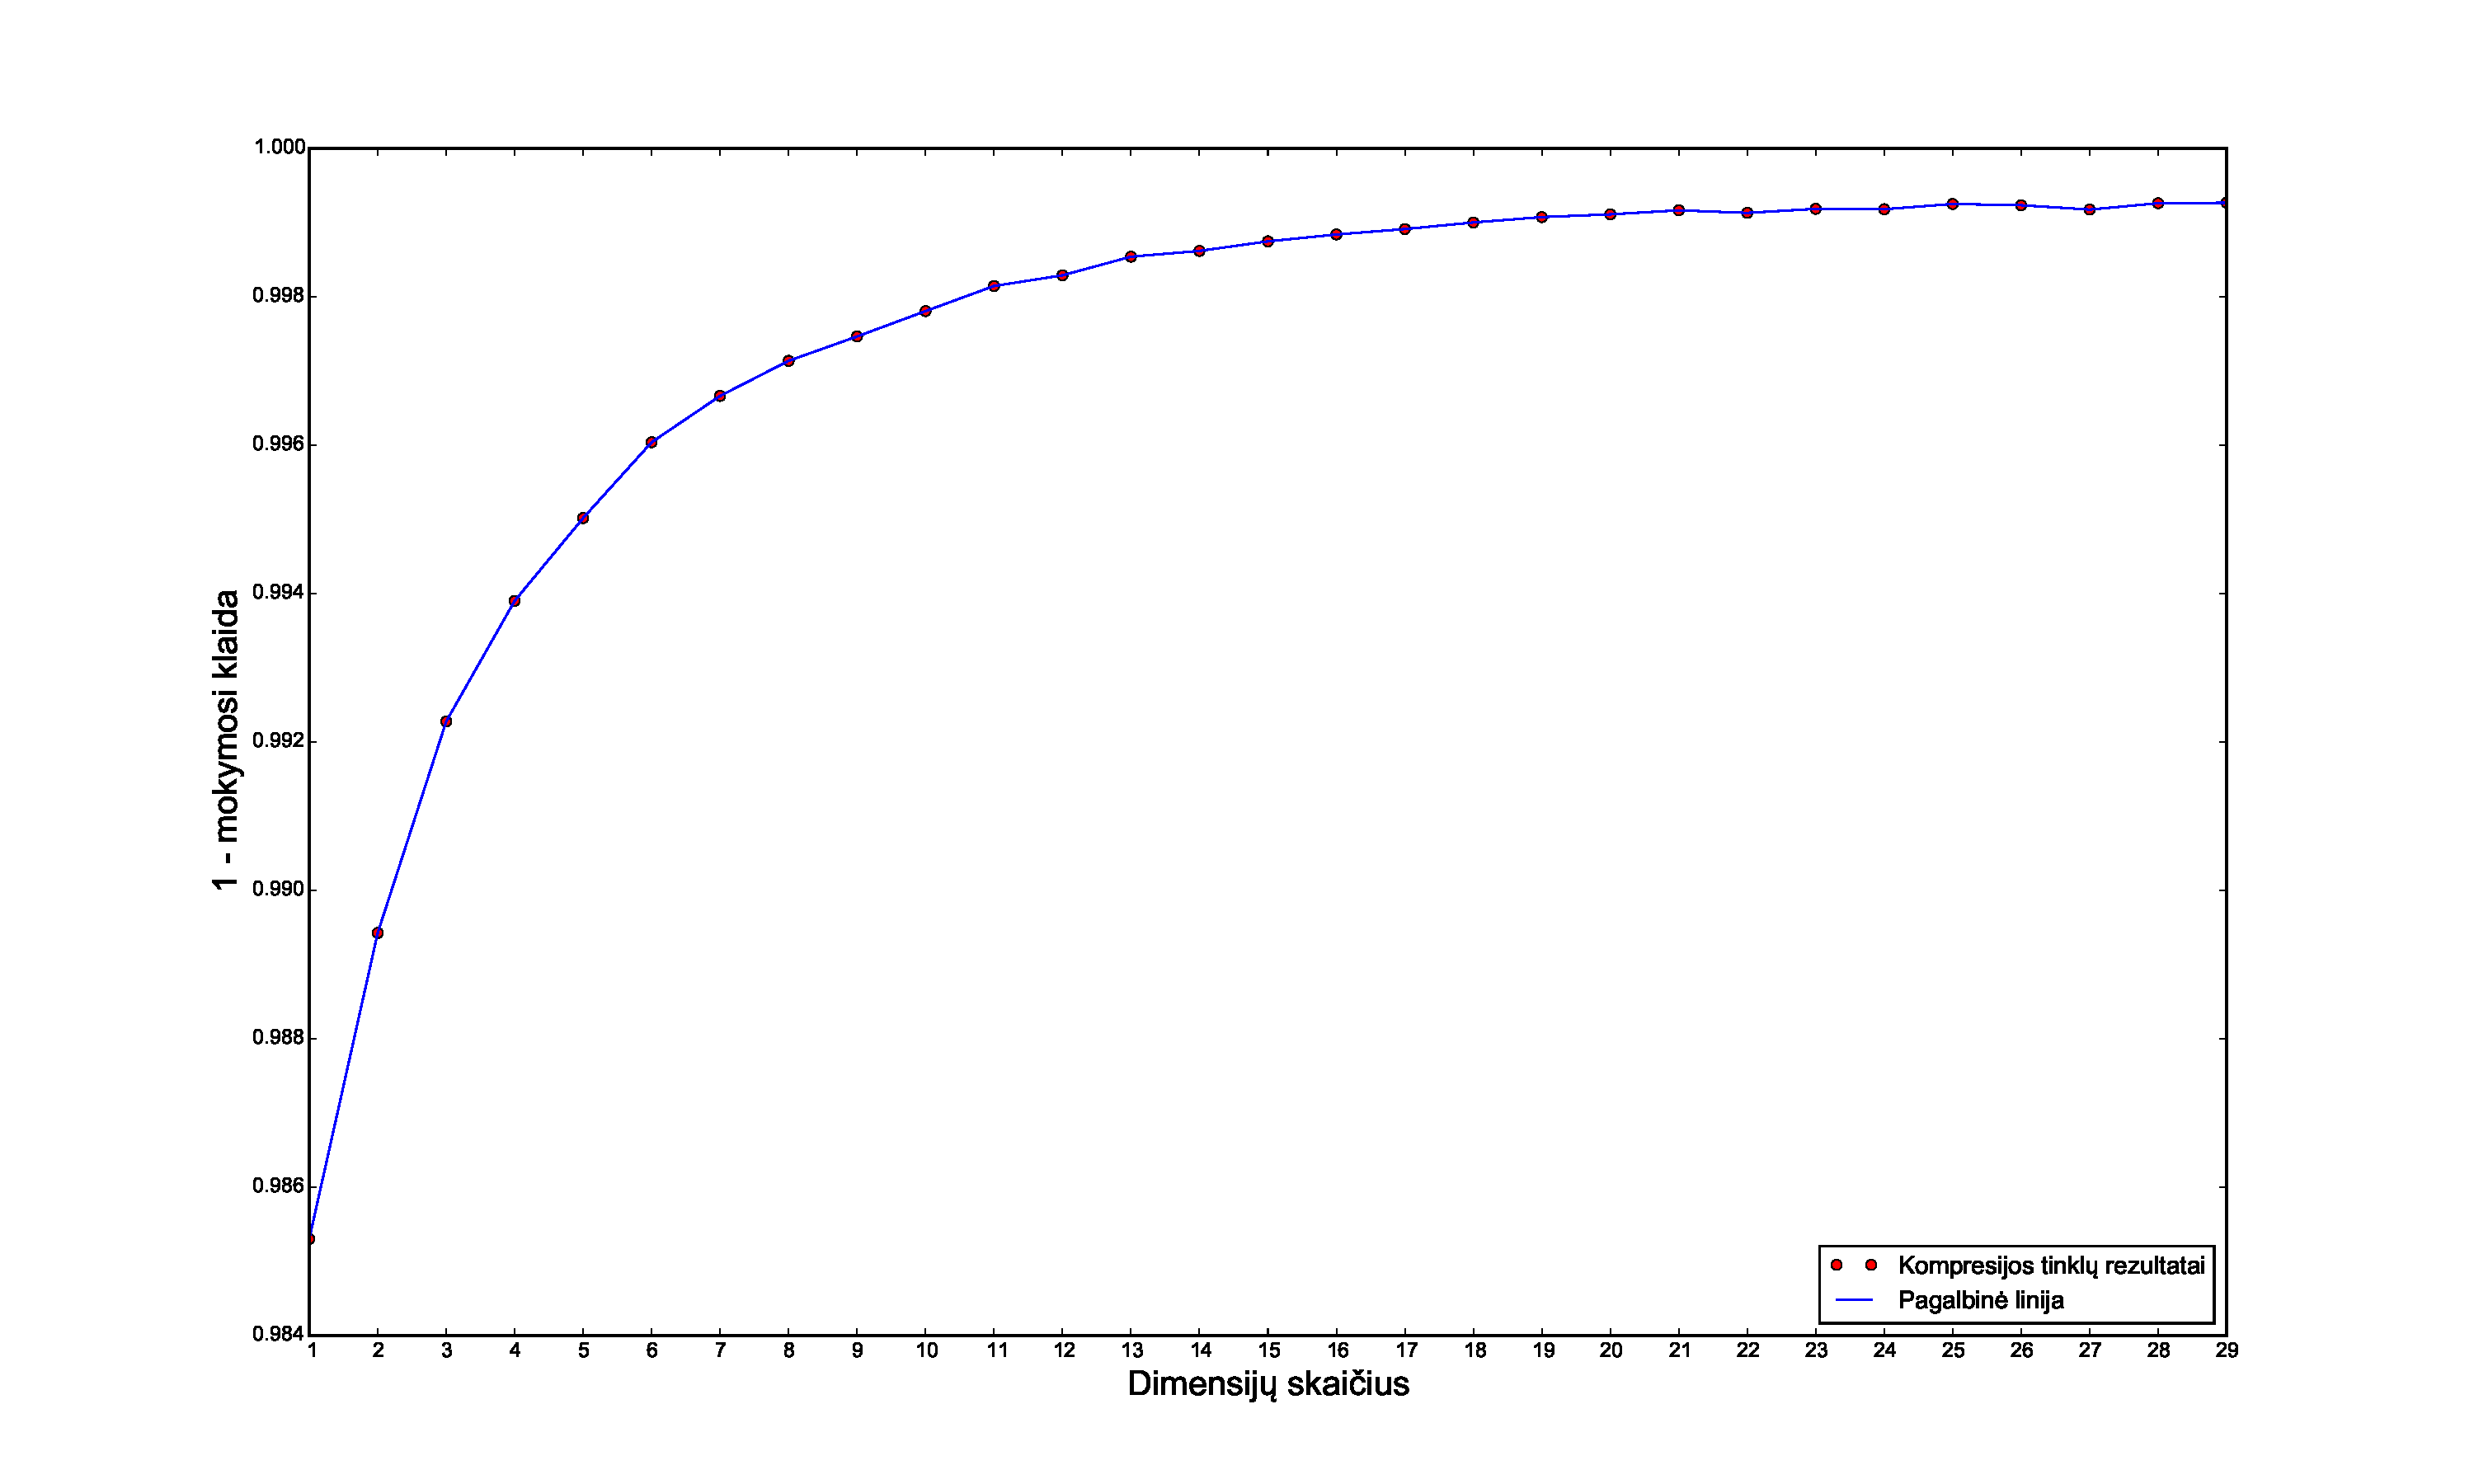
\includegraphics[scale=0.25]{pics/compression_dimensions}
	\caption{Duomenų kompresijos rezultatai}
	\label{fig:compression_dimensions}
\end{figure}

Tiriamų duomenų dimensiškumas buvo sumažintas šiuo būdu.
Buvo paimta po 500 įrašų iš 3 skirtingų grupių.
Kadangi duomenys turi 30 dimensijų, duomenų dimensijos buvo mažinamos iki [1; 29] dimensijų.
Gauti rezultatai pavaizduoti \ref{fig:compression_dimensions}~pav.
Rezultatuose matoma, kaip tiksliai daugiasluoksnis kompresijos perceptronas geba atstatyti pradinius 30 dimensijų duomenis turėdamas sukompresuotus mažiau dimensijų turinčius duomenis.
Galima pastebėti, kad mažėjant dimensijų skaičiui, atstatyti pradinius duomenis darosi vis sunkiau.
Visgi mažinant dimensijų skaičių iki tam tikros ribos, kompresijos teisingumas mažėja ganėtinai lėtai.
Tęsiant dimensijų mažinimą, teisingumas pradeda kristi vis greičiau.
Iš to galima daryti prielaidą, kad analizuojamuose duomenyse yra pasikartojančios ar tiesiogiai tarpusavyje priklausančios informacijos, kurią galima sukompresuoti į mažiau dimensijų turinčią ir naudingesnę informaciją.
Tačiau svarbu pasirinkti tinkamą dimensijų skaičių, kadangi pasirinkus per mažai dimensijų, kompresija gali prarasti didelę svarbios informacijos dalį.

\begin{figure}
	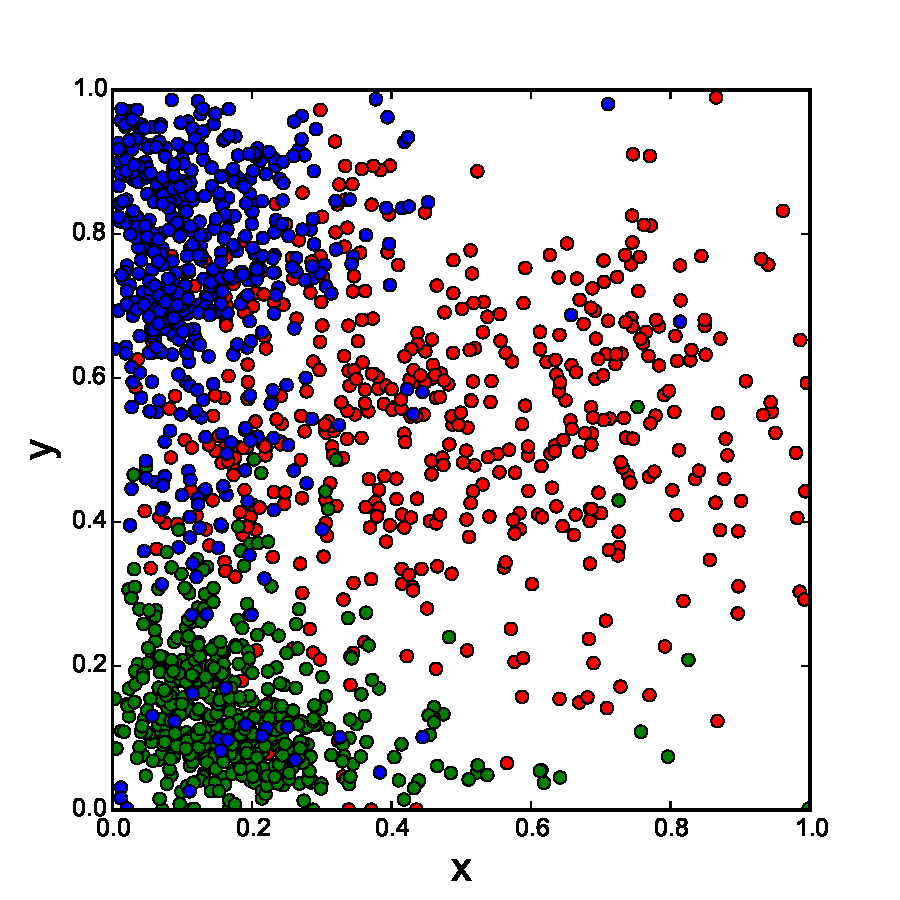
\includegraphics[scale=0.5]{pics/points_2d}
	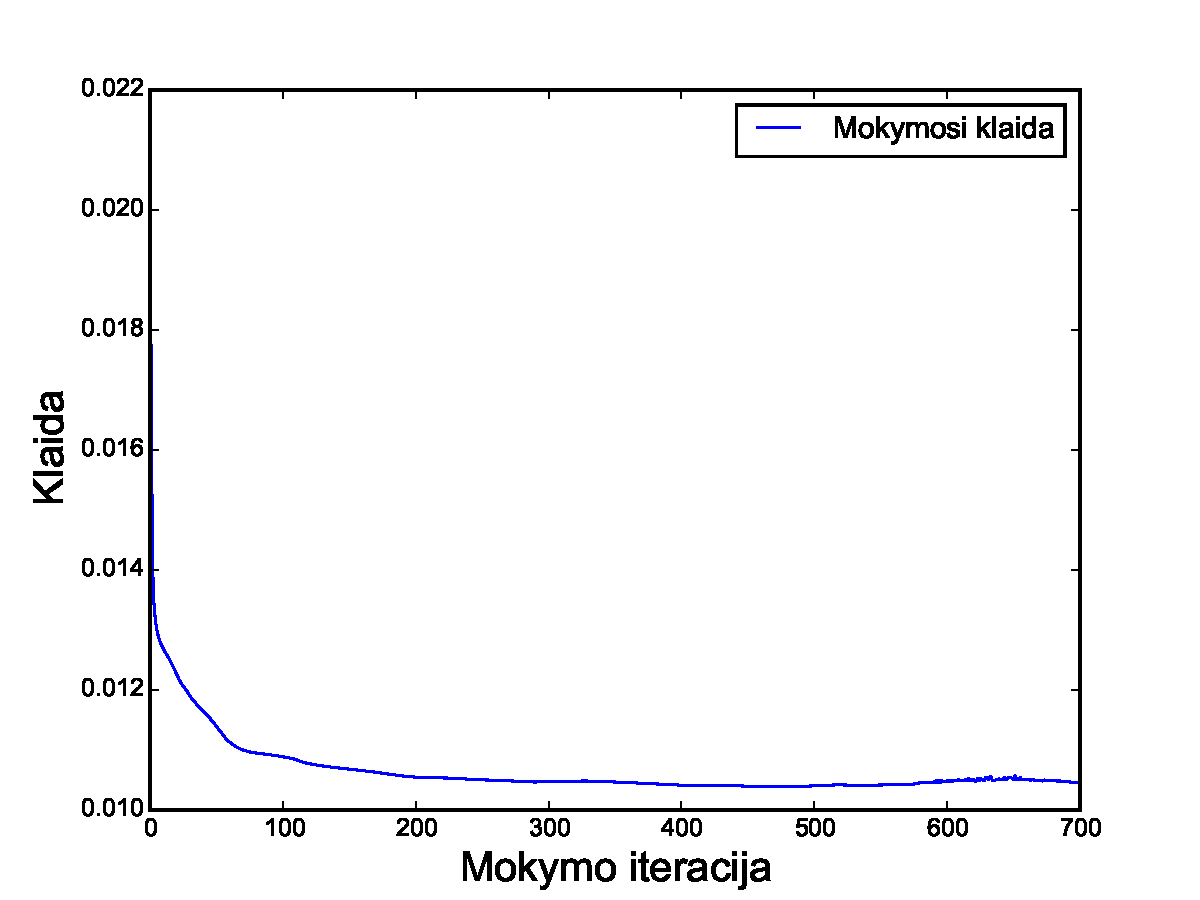
\includegraphics[scale=0.5]{pics/points_2d_progress}
	\caption{Dvimačiai duomenys}
	\label{fig:2d_points}
\end{figure}

\begin{figure}
	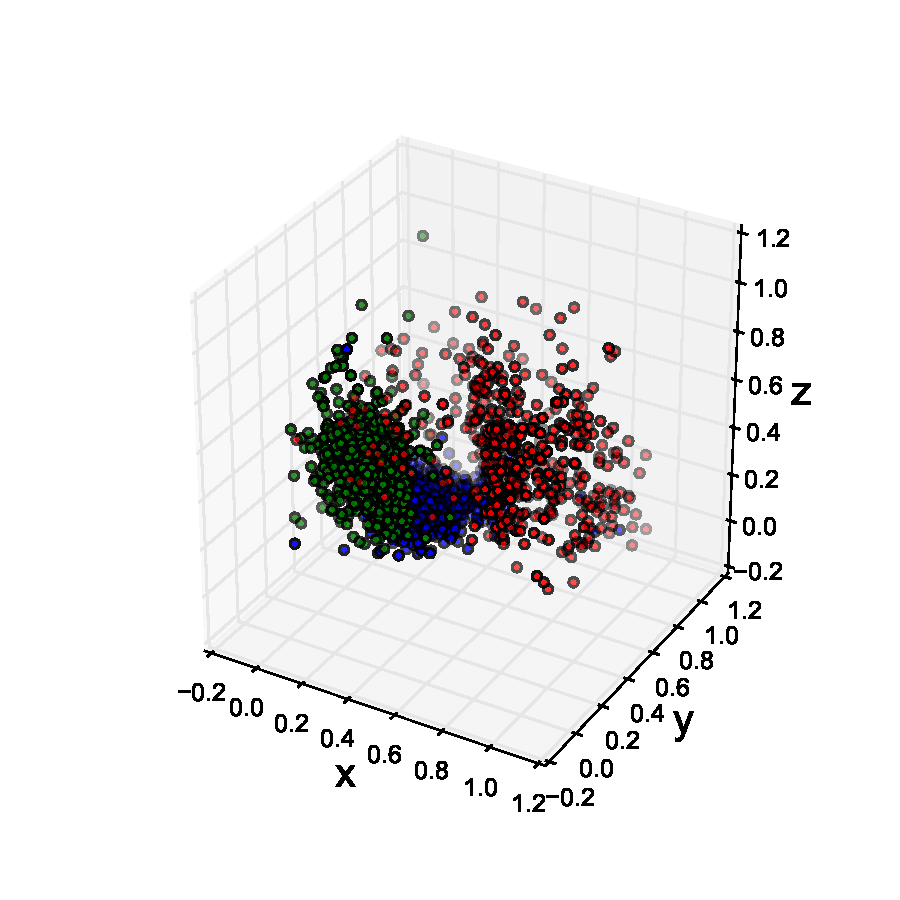
\includegraphics[scale=0.5]{pics/points_3d}
	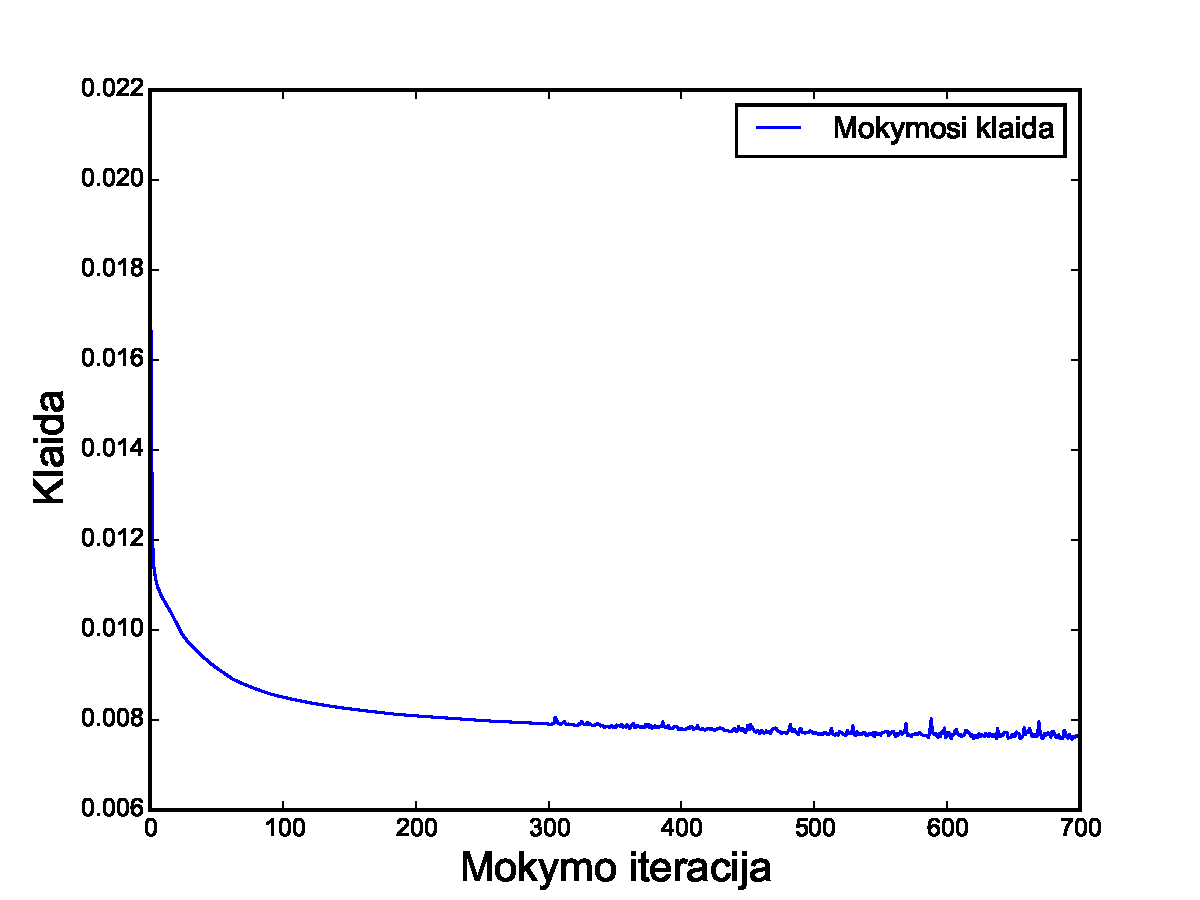
\includegraphics[scale=0.5]{pics/points_3d_progress}
	\caption{Trimačiai duomenys}
	\label{fig:3d_points}
\end{figure}

Pateikiami dvimačių (\ref{fig:2d_points}~pav.) ir trimačių (\ref{fig:3d_points}~pav.) duomenų kompresijos rezultatai - kairėje pusėje pavaizduoti sukompresuoti duomenys, skirtingų grupių įrašus pavaizduojant skirtingomis spalvomis, o dešinėje - tinklo apmokymo klaidos kitimo diagramos.
Iš pateiktų rezultatų matosi, kad dvimačiai duomenys susigrupavę ne taip gerai, kaip trimačiai.
Kadangi turimi duomenys turi 30 dimensijų, todėl dimensijų sumažinimas iki 2 praranda didesnę dalį duomenų nei mažinant iki 3 dimensijų.
Didesnių dimensijų kompresijos rezultatų vizualiai pavaizduoti nepavyksta dėl natūralių priežasčių.




\section{Klasifikavimas mažinant dimensiškumą}

Norint išsiaiškinti, ar galima pasiekti geresnius klasifikavimo rezultatus prieš tai sumažinant duomenų dimensiškumą, buvo atliktas tyrimas.
Kadangi tiriamus duomenis sudaro 30 dimensijų, buvo bandoma sumažinti dimensijas iki visų galimų dimensijų dydžių - nuo 1 iki 29.
Norint išsiaiškinti klasifikavimo efektyvumą pasirinkus į kiek dimensijų bus kompresuojami duomenys, atliekamas eksperimentas.

Eksperimento metu pirmiausia sukuriamas ir apmokomas daugiasluoksnis perceptronas, skirtas kompresuoti duomenis į pasirinktą dimensijų skaičių.
Šį perceptroną sudaro 5 sluoksniai - įvedimo, išvedimo bei 3 paslėptieji sluoksniai.
Įvedimo, išvedimo bei 2 paslėptieji sluoksniai turi po 30 neuronų.
Trečiasis paslėptasis sluoksnis, esantys tinklo viduryje, turi tiek neuronų, į kiek dimensijų norima sukompresuoti duomenis - pagal \ref{dimensionality-reduction-perceptron} poskyryje aprašytą metodą šiame sluoksnyje ir yra gaunami sukompresuoti duomenys.
Šis sluoksnis tada yra apmokomas 300 kartų iteruojant per visus mokymo rinkinio įrašus.
Apmokius tinklą, duomenys yra sukompresuojami pasinaudojant geriausią mokymo metu pasiektą rezultatą.

Gavus sukompresuotus duomenis, pradedamas klasifikavimas.
Pirmiausia sukuriamas klasifikavimui skirtas daugiasluoksnis perceptronas.
Šį perceptroną sudaro 4 sluoksniai.
Pirmasis - įvesties sluoksnis, turintis tiek neuronų, kiek dimensijų turi sukompresuoti duomenys.
Tada du paslėpti sluoksniai, turintys po 30 neuronų.
Galiausiai, išvesties sluoksnis, turintis tiek neuronų, kiek yra skirtingų galimų klasių.
Kadangi šio eksperimento metu buvo analizuojami duomenys iš 3 skirtingų klasių, todėl išvesties sluoksnis turėjo 3 neuronus.
Šis tinklas buvo apmokomas panaudojant iš kompresijos tinklo gautais kompresuotais duomenimis.
Apmokymas vyko 400 kartų, kaskart mokymo metu panaudojant visus mokymo rinkinio įrašus.
Baigus apmokymą, gaunamas rezultatas - klasifikavimo klaida.

Kiekvienam galimam dimensijų skaičiui, į kurį norima sutraukti duomenis, šis eksperimentas buvo atliktas po kelis kartus.
Taip buvo užtikrinama, kad gauti rezultatai bus patikimesni, kadangi kai kuriais atvejais atsitiktinai sugeneruoto perceptrono struktūra gali būti labai nepalanki ir gali būti gaunamas prastas rezultatas, neparodantis, kiek visgi toks kompresijos mažinimas gali padėti klasifikavimui.


\subsection{Kompresuotų duomenų klasifikavimo perceptronų galimybių eksperimentas}

Pirmiausia šis eksperimentas buvo atliktas su daliniais duomenimis.
Iš kiekvienos grupės paimta po 50 įrašų, kurie buvo naudojami eksperimentuose tiek apmokymui, tiek ir pačiam tinklo klaidos skaičiavimui.
Taip buvo pasielgta norint išsiaiškinti perceptronų galimybes - kadangi visi duomenys, kurie naudojami klaidos skaičiavime, yra naudojami taip pat ir apmokant, neuroniniui tinklui nelieka nežinomų duomenų.
Pirmiausia šie duomenys buvo panaudoti apmokant kompresijos tinklą, kuris po to buvo panaudotas šiems duomenims sukompresuoti.
Tada šie sumažinto dimensiškumo duomenys buvo panaudoti klasifikavimo tinklo apmokymui.
Apmokius klasifikavimo tinklą, gaunama klaida.
Tai atlikus po 5 kartus visiems galimiems dimensijų skaičiams, gauti rezultatai, pavaizduoti \ref{fig:experiment-1}~pav.

\TODO{paaiškinti grafiką}

\begin{figure}
	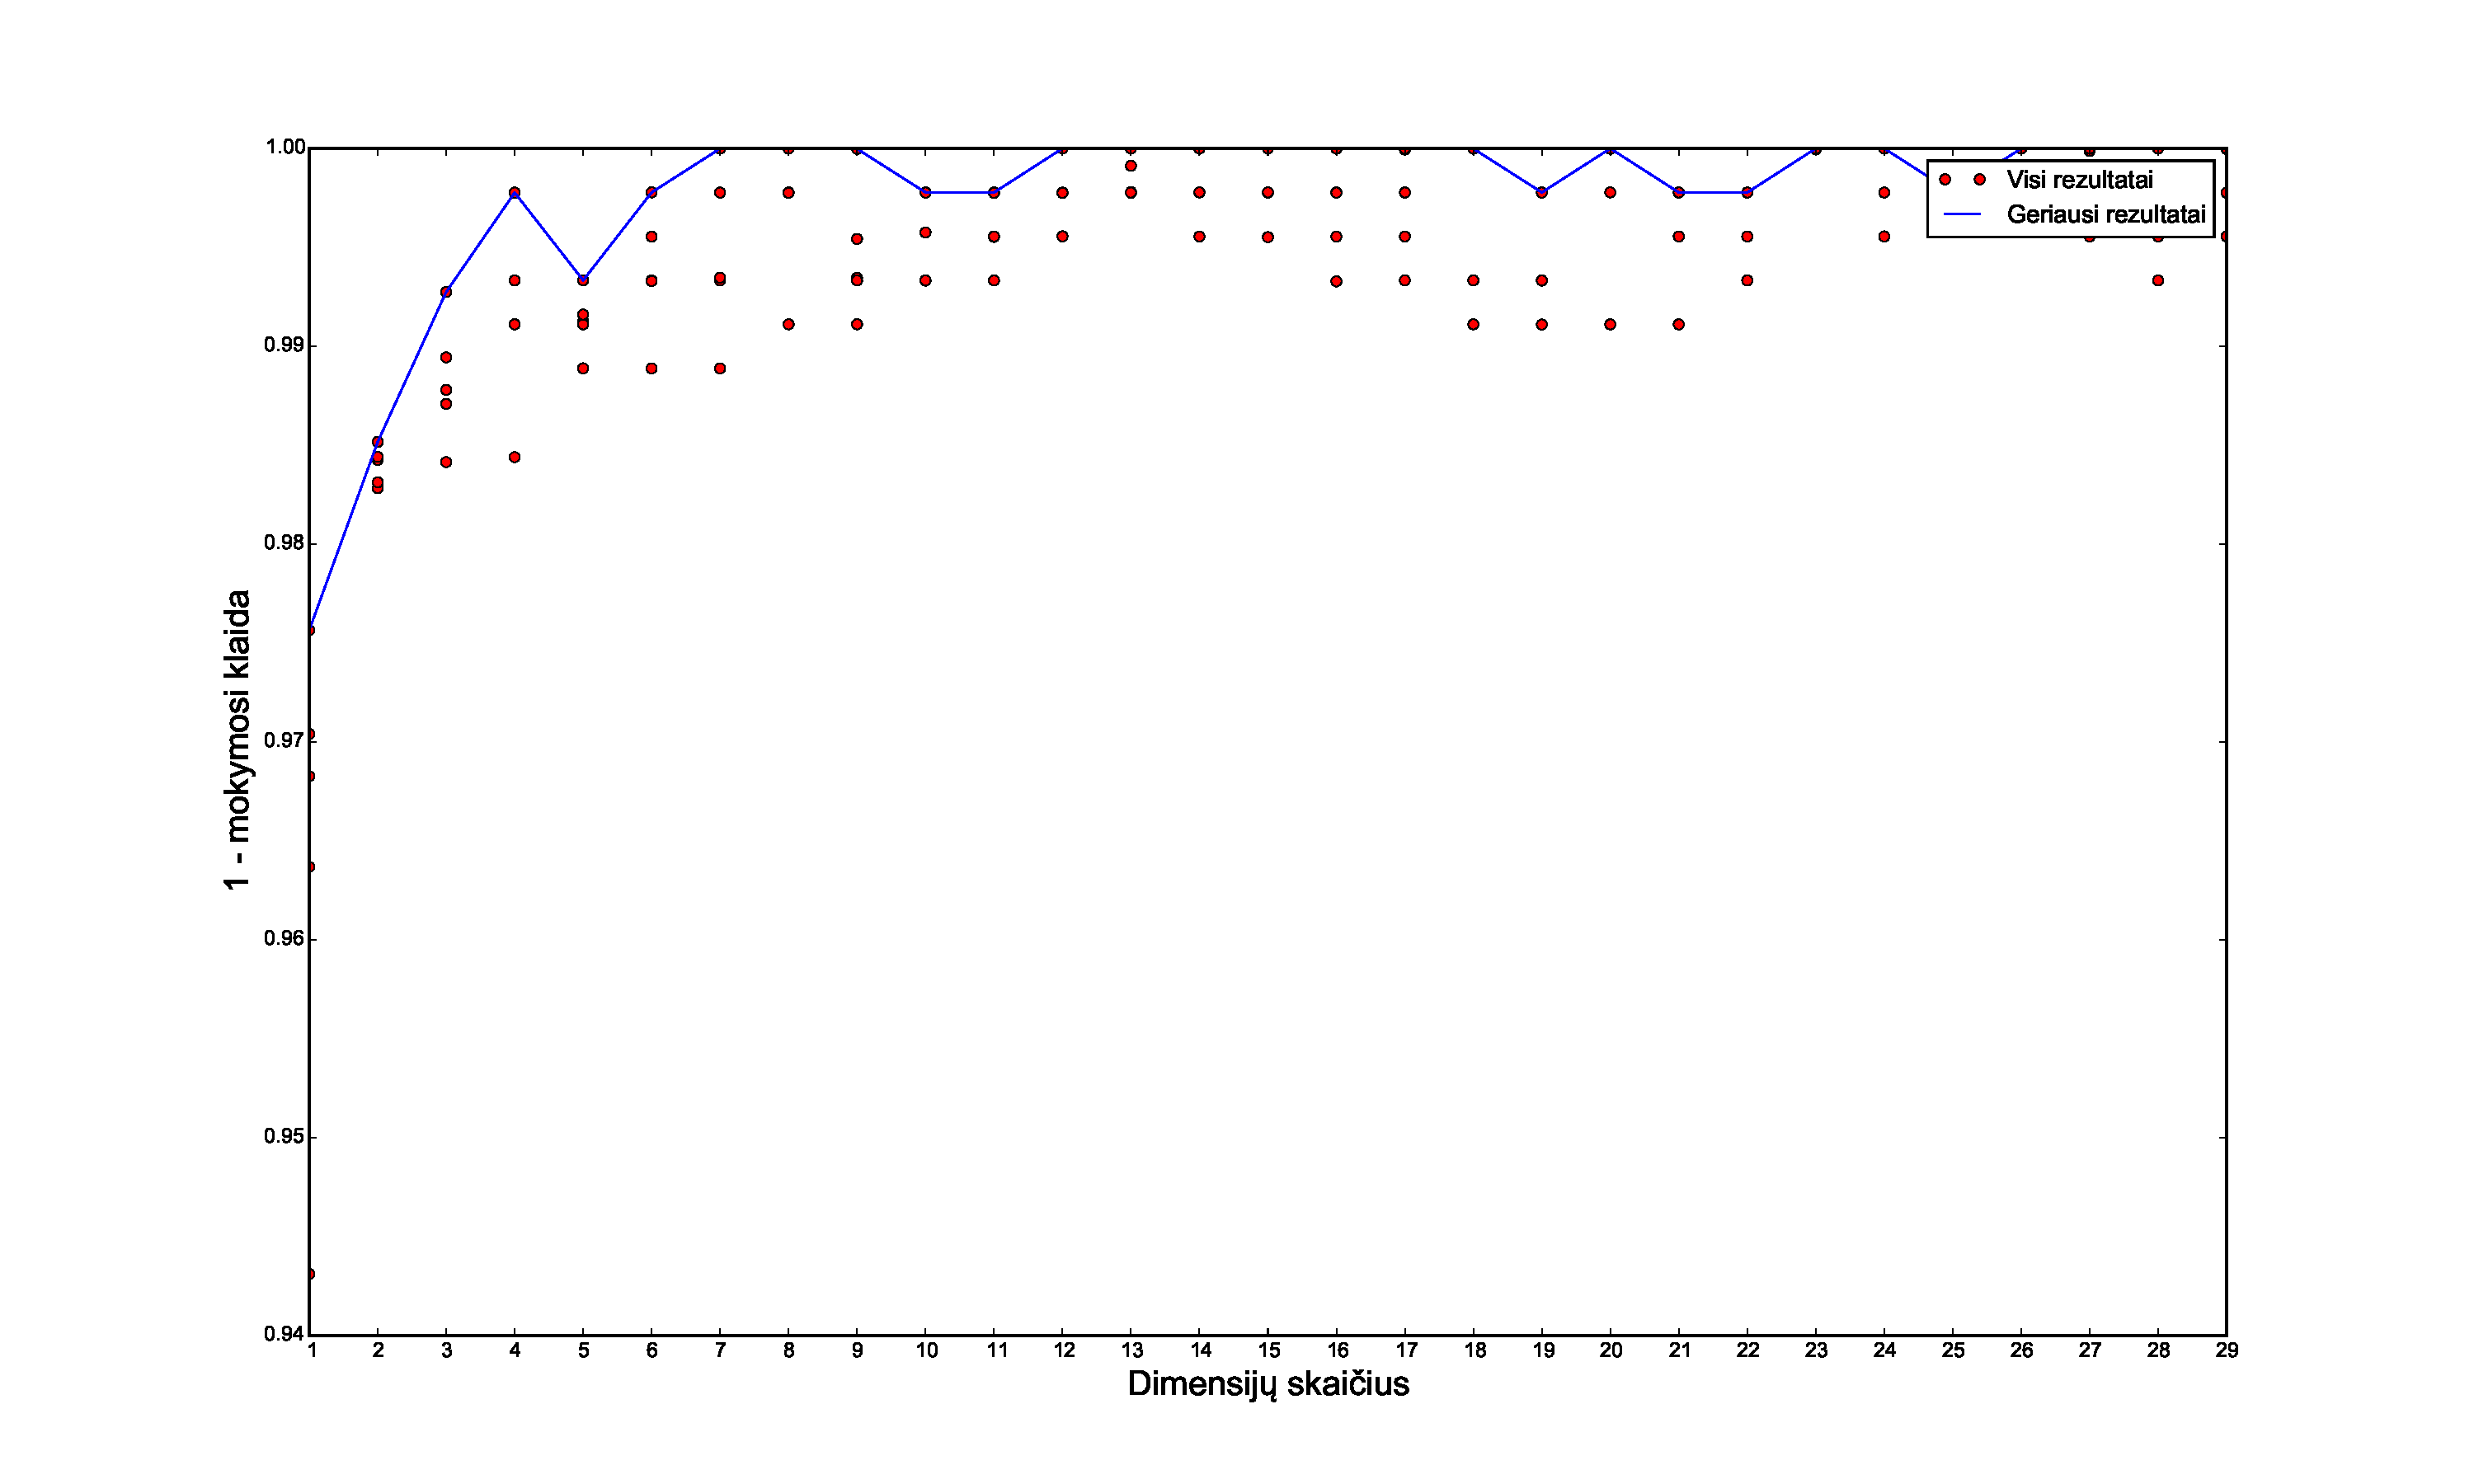
\includegraphics[scale=0.32]{pics/dimensions_2015-5-23_15-50-6}
	\caption{Klasifikavimo mažinant dimensijas rezultatai}
	\label{fig:experiment-1}
\end{figure}

Iš rezultatų matosi, kad klasifikavimo tinklas gerai geba susidoroti su tokiais mažais duomenimis - rezultatai labai netoli vieneto, tai yra, klaida beveik lygi nuliui.
Išimtis tyrimuose su mažais dimensijų skaičiais - kai dimensijų yra mažai, neuronų tinklas nesugeba suklasifikuoti sukompresuotų duomenų.
Tai parodo, kad mažinant dimensijų skaičių iki labai mažo, prarandama dalis informacijos apie duomenis.
Dėl to juos klasifikuoti pasidaro sunkiau.
Todėl norint padidinti klasifikavimo efektyvumą, dimensijų skaičių galima mažinti daugiausiai iki keturių.


\subsection{Kompresuotų duomenų klasifikavimo eksperimentas}

Sekančiame atliktame eksperimente buvo panaudoti visi įrašai iš tiriamų grupių - 500 įrašų iš 3 grupių.
Kompresijos perceptrono apmokymui buvo panaudoti visi šie įrašai, kadangi tikslas yra kuo tiksliau ir autentiškiau sukompresuoti visus duomenis, o ne paruošti tinklą, kuris gebėtų kompresuoti dar tinklui nematytus duomenis.
Apmokius kompresijos tinklą, gaunami kompresuoti duomenys.
Tada iš kiekvienos grupės atsitiktinai pasirenkama po 50 įrašų, kurie naudojami klasifikavimo perceptrono apmokymui.
Apmokius perceptroną, jo klaida skaičiuojama su visais duomenimis, o ne tik naudotais mokymo metu.
Taip dauguma įrašų perceptronui yra nauji, todėl taip ištiriama, kaip gerai perceptronas sugebėjo išmokti duomenų savybes iš mažų mokymo grupių.
Eksperimentas buvo atliktas kiekvienam dimensijų skaičiui po 30 kartų, norint užtikrinti kuo mažesnį atsitiktinumą.
Gauti rezultatai, pavaizduoti \ref{fig:experiment-2}~pav.

Iš šių rezultatų matosi, kad su pakankamai mažais dimensijų skaičiais (mažesniais nei 13), klasifikavimo perceptronas gauna šiek tiek didesnę klaidą nei su likusiais dimensijų skaičiais.
Taip turbūt atsitinka dėl panašių priežasčių, kaip ir pirmame tyrime su dimensijų skaičiais nuo vieno iki trijų - kompresija praranda dalį svarbios duomenų informacijos.
To nesimato pirmame eksperimente, kadangi skirtumai gan maži - blogiausias tyrimas pasiektas su 5 dimensijomis, kurio metu gauta klaida apie $1 - 0.965 = 0.035$.
Tuo tarpu praeitame eksperimente, kuriame buvo ištirti dar mažesni dimensijų skaičiai, blogiausias tyrimas pasiektas su viena dimensija, kurio klaida apie $1 - 0.943 = 0.057$ beveik dvigubai didesnė.
Tai didelis skirtumas žinant, kad pirmame eksperimente klaidos skaičiavimui buvo naudojami visi apmokymui naudoti duomenys.
Geriausi rezultatai gauti $[14; 29]$ dimensijų skaičiaus intervale.
Šio eksperimento metu patikimiausiai atrodo rezultatai su 18 dimensijų, todėl šis dimensijų skaičius buvo pasirinktas palyginimui.

\begin{figure}
	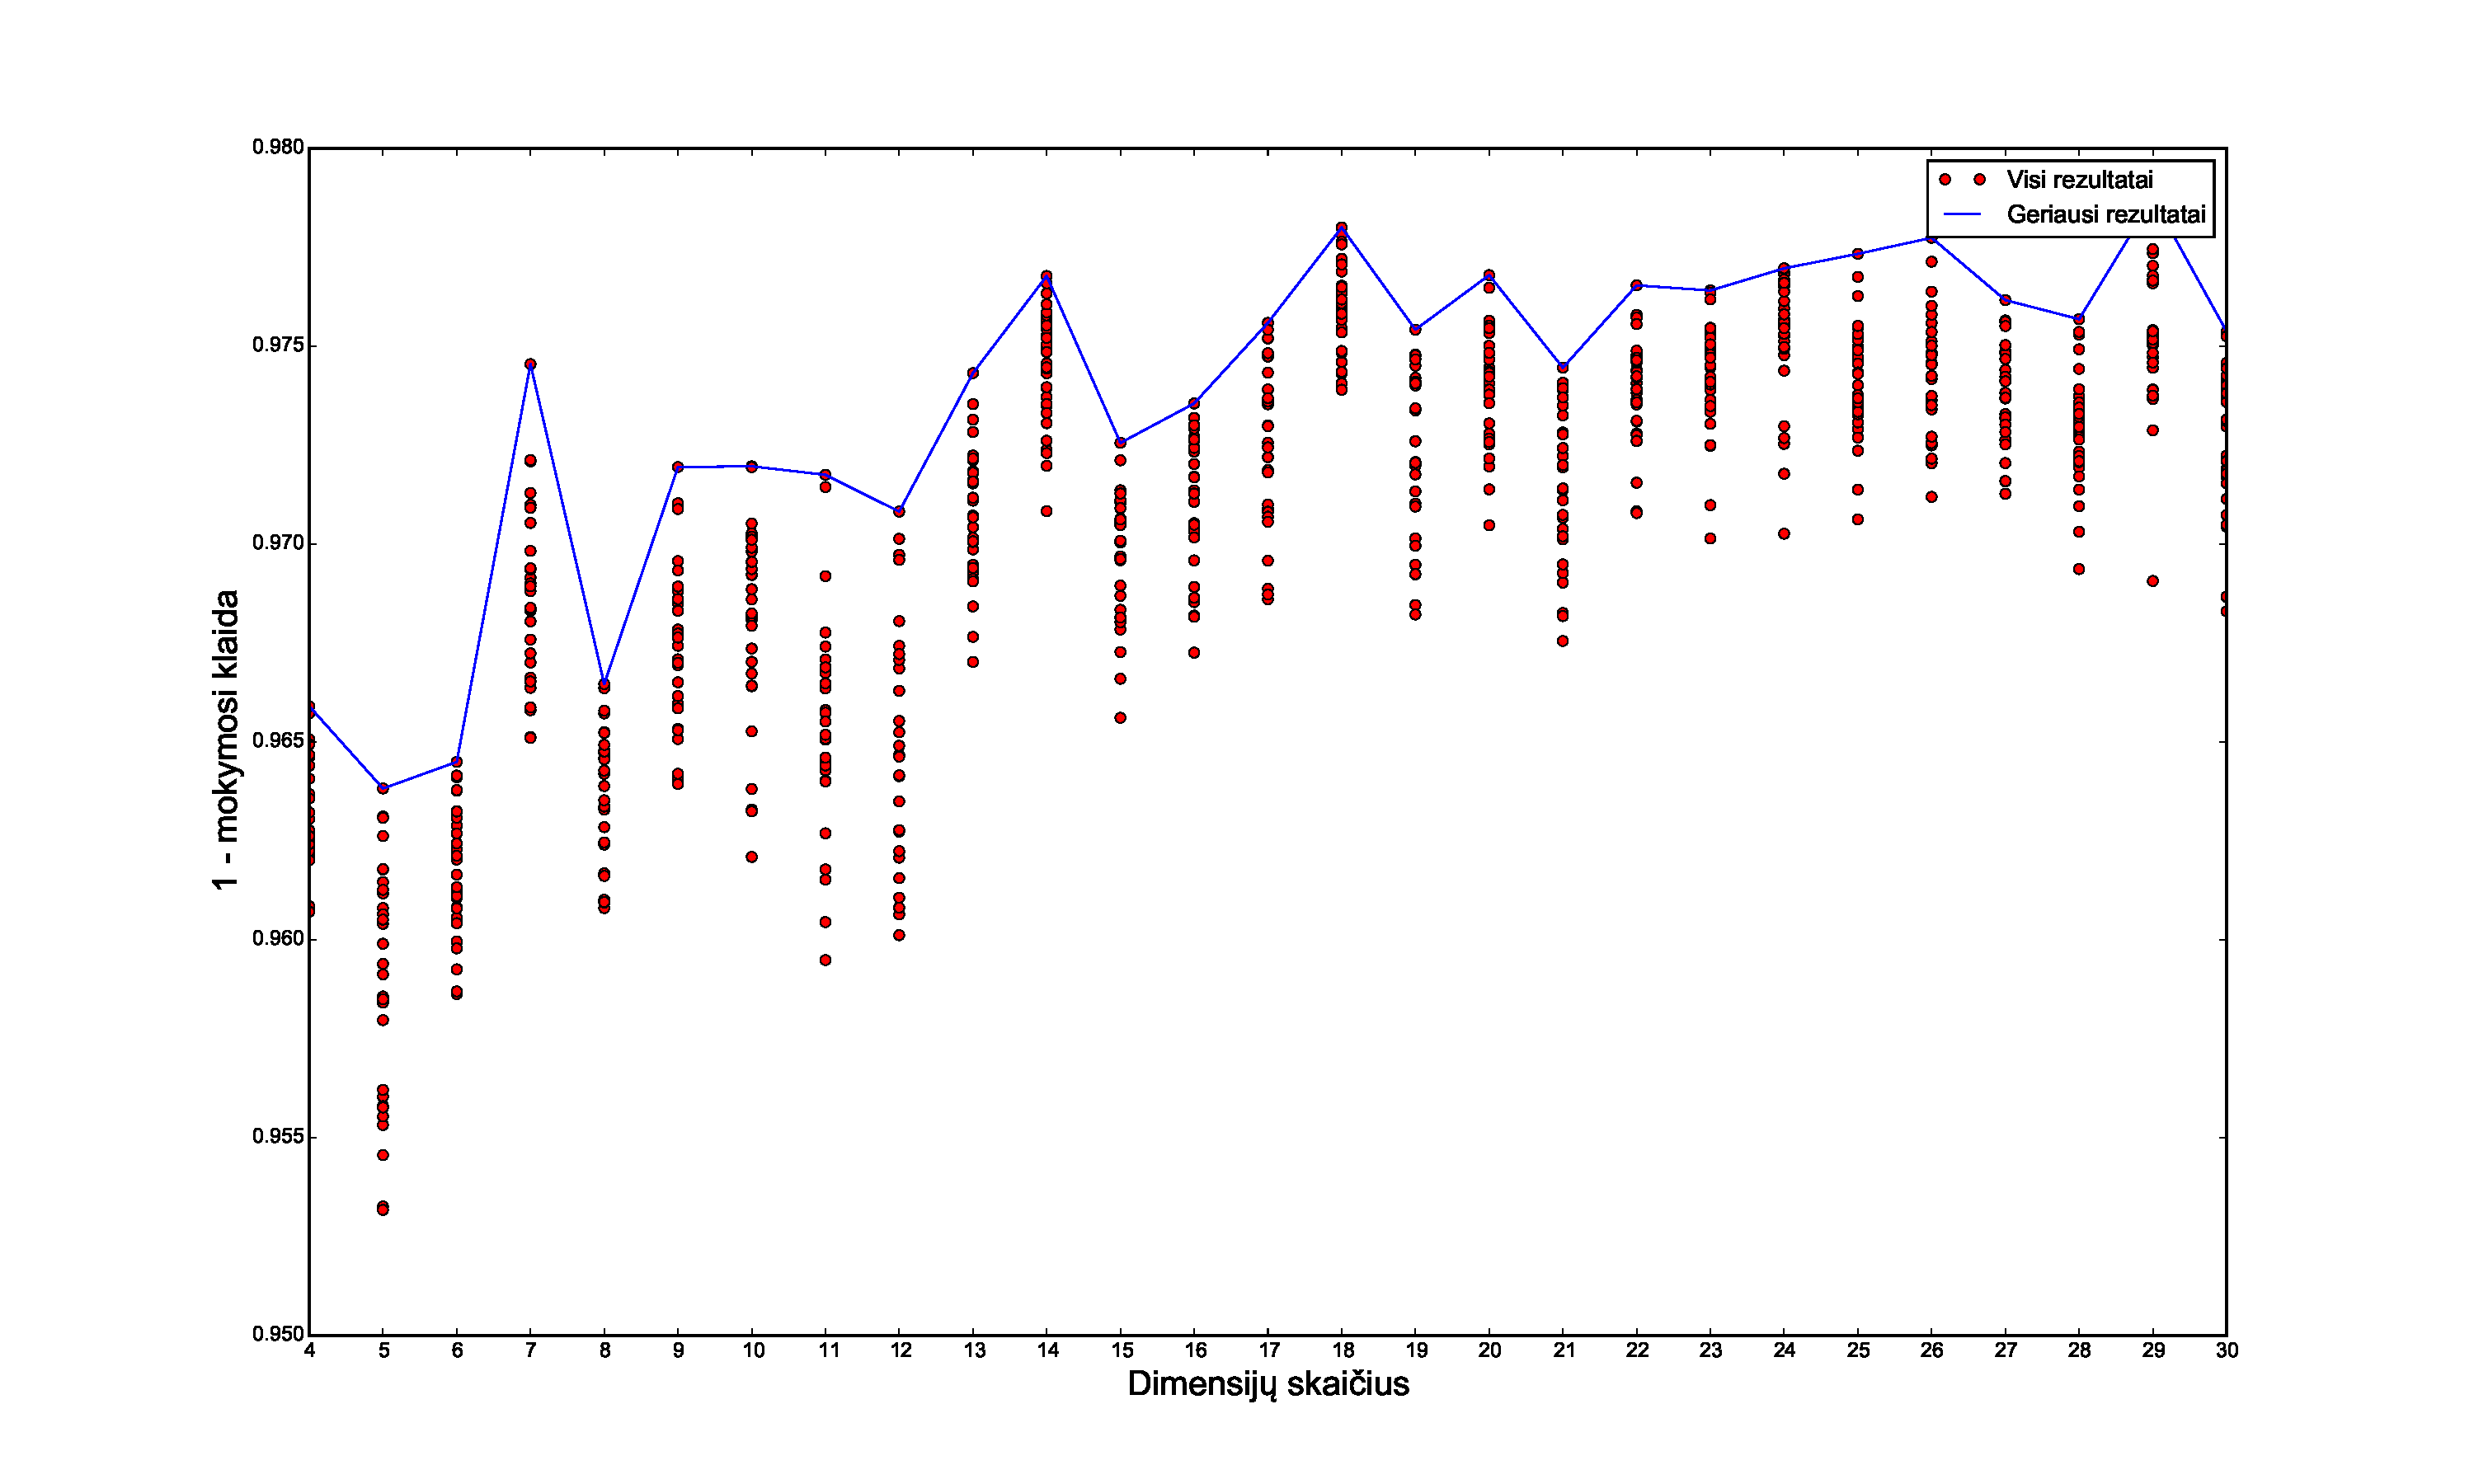
\includegraphics[scale=0.32]{pics/dimensions_2015-5-27_6-18-5}
	\caption{Klasifikavimo mažinant dimensijas rezultatai}
	\label{fig:experiment-2}
\end{figure}


\subsection{Originalių ir kompresuotų duomenų klasifikavimo palyginimas}

Buvo atliktas klasifikavimo efektyvumo palyginimas naudojant originalius 30-ties dimensijų bei kompresuotus 18-os dimensijų duomenis.
Palyginimui buvo naudojami tie patys duomenys - po 500 įrašų iš kiekvienos grupės, ir tik po 50 iš jų naudojami apmokymui (validacijai buvo panaudoti visi 500 įrašų iš kiekvienos grupės).
Gautas rezultatai pavaizduotas \ref{fig:dim-comparisons}~pav.

\begin{figure}
	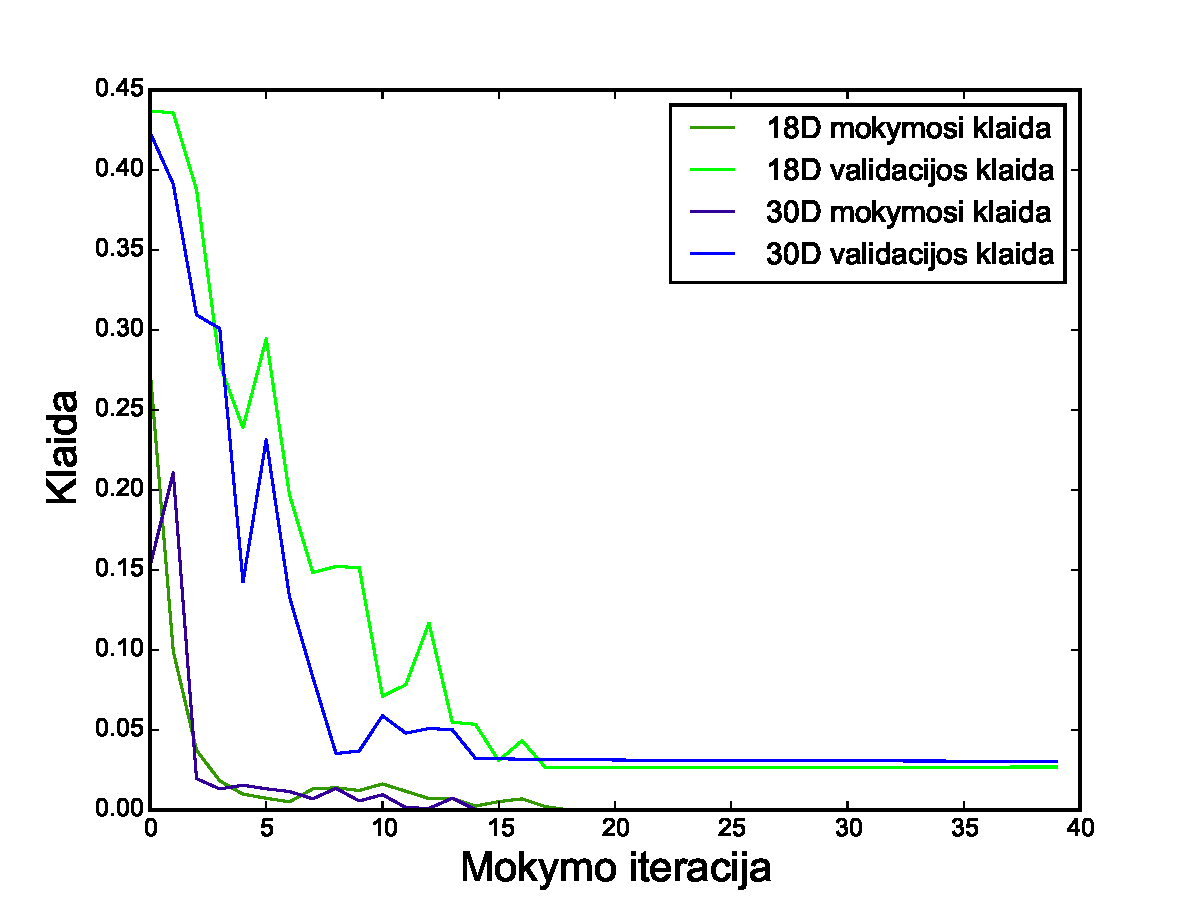
\includegraphics[scale=0.75]{pics/dim_comparisons_2015-5-27_14-21-13}
	\caption{18 ir 30 dimensijų klasifikavimo palyginimas}
	\label{fig:dim-comparisons}
\end{figure}

Iš rezultato matosi, kad abu klasifikavimo perceptronai sugebėjo pasiekti beveik nulinę klaidą mokymo procese.
Tai reiškia, kad perceptronai pilnai išmoko mokymui naudotus duomenis ir daugiau pastebimai tobulėti negali.
Visgi galutinė validacijos klaida skiriasi - 18-os dimensijų duomenų validacijos klaida mažesnė už 30-ties.


\sectionnonum{Rezultatai ir išvados}
Rezultatų ir išvadų dalyje išdėstomi pagrindiniai darbo rezultatai (kažkas
išanalizuota, kažkas sukurta, kažkas įdiegta), toliau pateikiamos išvados
(daromi nagrinėtų problemų sprendimo metodų palyginimai, siūlomos
rekomendacijos, akcentuojamos naujovės). Rezultatai ir išvados pateikiami
sunumeruotų (gali būti hierarchiniai) sąrašų pavidalu. Darbo rezultatai turi
atitikti darbo tikslą.

\TODO{Suprogramuotas neuroninis tinklas}
\TODO{Išanalizuoti duomenys}
\TODO{Išbandyti skirtingi dimensiškumo mažinimo metodai}
\TODO{Išbandyti skirtingi klasifikavimo metodai}
\TODO{Išbandyti skirtingi dimensiškumo mažinimo ir klasifikavimo apjungimo metodai}


\printbibliography[heading=bibintoc]  % Šaltinių sąraše nurodoma panaudota
% literatūra, kitokie šaltiniai. Abėcėlės tvarka išdėstomi darbe panaudotų
% (cituotų, perfrazuotų ar bent paminėtų) mokslo leidinių, kitokių publikacijų
% bibliografiniai aprašai. Šaltinių sąrašas spausdinamas iš naujo puslapio.
% Aprašai pateikiami netransliteruoti. Šaltinių sąraše negali būti tokių
% šaltinių, kurie nebuvo paminėti tekste. Šaltinių sąraše rekomenduojame
% necituoti savo kursinio darbo, nes tai nėra oficialus literatūros šaltinis.
% Jei tokių nuorodų reikia, pateikti jas tekste.

% \sectionnonum{Sutartinis terminų žodynas}
% Sąvokų apibrėžimai ir santrumpų sąrašas sudaromas tada, kai darbo tekste
% vartojami specialūs paaiškinimo reikalaujantys terminai ir rečiau sutinkamos
% santrumpos.

\end{document}
